\documentclass{article}

\usepackage[utf8]{inputenc}

\usepackage{amsmath, bm}
\usepackage{graphicx}
\usepackage{amssymb}
\usepackage{float}
\usepackage{caption}
\usepackage{subcaption}
\usepackage{hyperref}
\usepackage{tikz}
\usepackage{layout}
\usepackage{booktabs}

\usepackage[margin=1in]{geometry}
\usepackage{listings}
\usepackage{xcolor}
\usepackage{color, colortbl}
\usepackage{textgreek}
\usepackage{mathrsfs}
\usepackage{savetrees}

\usetikzlibrary{calc}
\usetikzlibrary{angles,quotes} % for pic
\usetikzlibrary{patterns,snakes}
\usetikzlibrary{arrows}
\tikzset{>=latex} % for LaTeX arrow head

\setlength{\parskip}{\baselineskip}%
\setlength{\parindent}{0pt}%
\linespread{0.9}


\definecolor{codegreen}{rgb}{0,0.6,0}
\definecolor{codegray}{rgb}{0.5,0.5,0.5}
\definecolor{codepurple}{rgb}{0.58,0,0.82}
\definecolor{backcolour}{rgb}{0.95,0.95,0.92}

\lstdefinestyle{mystyle}{
    backgroundcolor=\color{backcolour},   
    commentstyle=\color{codegreen},
    keywordstyle=\color{magenta},
    numberstyle=\tiny\color{codegray},
    stringstyle=\color{codepurple},
    basicstyle=\ttfamily\footnotesize,
    breakatwhitespace=false,         
    breaklines=true,                 
    captionpos=b,                    
    keepspaces=true,                 
    numbers=left,                    
    numbersep=5pt,                  
    showspaces=false,                
    showstringspaces=false,
    showtabs=false,                  
    tabsize=2
}

\lstset{style=mystyle}



\begin{document}

\title{Computational Fluid Dynamics \\
    \large Interim Report}
\author{lwp26}
\date{October 2024}
\maketitle 

\iffalse
\begin{abstract}
    \centering

\end{abstract}
\fi

%-----------------------------------------------------------------------------------------
\section{Introduction}
%-----------------------------------------------------------------------------------------

Computational Fluid Dynamics (CFD) is a powerful tool for solving fluid flow problems.
This can be done much faster and at lower cost than experimental methods.
This makes it a valuable tool to be used alongside experimental validation.

\section{Objective}

To write a program to solve the Euler equations for two-dimensional flows using a finite volume time
marching method. Completing this work will give you practical expertise in pre-processing and post-
processing the simulations as well as understanding the methods of solution. The knowledge gained
is core to all CFD methods and transferrable to all other research and commercial CFD packages

\section{Software}

The software is a Qt application that calls fortran routines to solve the Euler equations for a 2D inviscid flow.
The user interface is shown in Figure \ref{fig:ui} and consists of an input panel and console on the left,
a convergence plot in the middle, and various tabs for viewing grid data on the right.
The solver routine is ran in a seperate thread to allow the user to interact with graphs and the console while the solver is running.
Modifications made to the original code involved binding fortran types to C structs so they could be exchanged between the solver and gui threads to be plotted.
This also lays some of the groundwork for future parallelisation of the solver, which may be considered in the improvements if time allows.

Modifications were also made to the convergence criteria to stop the solver when the last 100 calculated $d_avg$ were all within 1\% of their mean.
This was done to prevent the solver from reaching max iterations when the solution had already converged, making it possible to measure the runtime.
However, this could cause the solver to stop prematurely if the convergence was slow, and so the tolerance of 1\% may need to be adjusted.
The original check if the final residual error is within the bounds specified in the inputs is nested within this check.
This means the solver subroutine will terminate with 4 possible outcomes:
\begin{itemize}
    \item Converged within boundary specified
    \item Converged outside boundary specified
    \item Diverged
    \item Maximum iterations reached
\end{itemize}

The measurement of runtime was done by averaging the time taken to run the solver over three runs.
This is necessary as for small runtimes, there can be significant variation due windows scheduling and other background processes.
The maximum number of iterations was set to 100,000 which is sufficient for most cases.
The convergence boundary specified in the input file was set to $10^{-4}$ for all cases.

A comparison of runtimes for different compiler flags was done to optimise the performance of the program and is shown in Table \ref{tab:performance}.
A faster program allows for a wider range and resolution of parameters to be tested for better analysis.
An additional python script was written to run the solver and save settings, runtime data and convergence data to a file.


\section{Discussion}

% Comment on the results from the above two test cases. Pay special attention to ways of
% assessing the accuracy of the solutions and further figures that you can create to analyse this

% Discuss the effects of varying CFL number, smoothing factor and mesh size. Examine how
% these choices affect accuracy, stability and runtime of the solver.


% for each figure
% explain trend
% explain magnitude
\subsection{Bump case}

Figure \ref{fig:bump_mach} shows the Mach number distribution over the bump domain.
The solution to the Euler equations for this case, which is absent of shocks, should be symmetrical about the center of the bump.
However, asymmetry is observed in the low mach number region to the right of the bump.
Figure \ref{fig:bump_cp} shows the pressure coefficient distribution over the bump domain, showing good agreement with
the Mach plot where regions of high pressure coincide with low Mach number regions.
A small smoothing factor was chosen for accuracy and a $CFL$ number close to the largest possible for stability  was used to ensure the solver made good progress.
The results match those in the handout closely \cite{handout}.

In figure \ref{fig:bump_conv} the convergence history of all the primary flow variables are shown.
The maximum residuals show a decrease in one order of magnitude over the first 20,000 iterations, after which these begin to plateau.
The averaged residuals decrease nearly two orders of magnitude and start to plateau at around 40,000 iterations.
Oscillations in the residuals were observed at low smoothing factors, which is expected as there is less dissipation of large gradients.
These oscillations were also observed for detailed meshes, which produce larger spatial gradient errors which must be dissipated over a smaller area each iteration.
High CFL numbers also cause oscillations as larger timesteps relative to the mesh size cause the solver to overshoot the solution, potentially amplifying the residuals.

Figure \ref{fig:bump_d_avg_cfl} shows the average density residual against the CFL number.
The CFL number is proportional to the timestep $\Delta t$, and by plotting the residuals against this parameter on a log-log plot, we can determine the order of the error.
This shows that our scheme is first-order time accurate.
Figure \ref{fig:bump_d_avg_ni} shows the average density residual against the number of cells in the $i$ direction.
The $n_i$ parameter is inversely proportional to the spatial step size $\Delta x$.
The graph shows the scheme is second-order spatially accurate for smaller mesh sizes, but the error plateaus for larger meshes.
This is due to floating point errors limiting the accuracy of area and spatial derivatives.
A deviation from the expected second-order convergence is also observed for the smallest mesh size,
which is due to boundary conditions applied at large scales. 

Figure \ref{fig:bump_time_cfl} shows log runtime against the CFL number.
This shows that the runtime is inversely proportional to the square of the CFL number, meaning that quartering the CFL doubles the runtime.
The number of iterations required to converge is inversely proportional to the CFL number.
Figure \ref{fig:bump_time_ni} shows the log runtime against log $n_i$.
The line shows proportionality at higher mesh sizes with higher runtimes at smaller mesh sizes.
This is likely due to increased and unstable errors failing to meet the convergence criteria.

Figure \ref{fig:bump_cfl_sfac_residual} shows a scatter plot of runs with varying CFL and smoothing factor.
The marker shape indicates termination status, with the colour indicating the Log average density residual.
The plot shows that at high CFL numbers and low smoothing the solver diverges.
This is because instabilities that arise from the high CFL numbers are not dissipated by the artificial smoothing.
Improved accuracy in the form of reduced error residuals are achieved at lower CFL and smoothing factors.
The similar plot, figure \ref{fig:bump_cfl_sfac_time} shows that this improved accuracy comes at the cost of increased runtime.

The figure \ref{fig:bump_ni_cfl_residual} is a similar scatter plot but varying $CFL$ and $n_i$.
It shows that an increased mesh detail, a slightly smaller CFL number is required for stability.
This is for reasons mentioned earlier, where larger spatial gradient errors must be dissipated over a smaller area each iteration.
The plot contains some incorrectly marked converged runs in the top left where the average error very slowly increased, indicating instability.
This highlights an issue with the convergence criteria, which needs to be refined to prevent premature termination.
Figure \ref{fig:bump_ni_cfl_time}, then shows that increasing this mesh detail improves accuracy at the cost of runtime.

\subsection{Bend case}

The bend case mach number distribution is shown in figure \ref{fig:bend_mach}.
A region of supersonic flow can be seen on the inside of the bend by the Mach 1 contour, which seems to compress back to subsonic flow before re-expanding to supersonic just before the exit.
The corresponding static pressure distribution is shown in figure \ref{fig:bend_cp}.
A small smoothing factor was chosen for accuracy and a correspondingly small CFL number was used to ensure the solver did not diverge.
The results differ slightly from the handout \cite{handout}, where the regions of supersonic flow in my run case are larger.
The final average density residual reached by the example in the handout is $3\times 10^{-5}$, where as my run case reached $5\times 10^{-6}$.
This suggests that my result is more accurate than that seen in the handout.

Figure \ref{fig:bend_conv} shows the convergence history, which shows more severe initial transience than the bump case, suggesting more innacuracies in the initial flow guess for this case.
Orders of error and runtime with respect to CFL and mesh size showed the same trends as with the bump case and so are omitted.

Figure \ref{fig:bend_cfl_sfac_residual} shows similar trends to the scatter plot for the bump case shown in figure \ref{fig:bump_cfl_sfac_residual}.
However, the line between converged and diverged is higher, indicating more smoothing is required for the bend case.
This could be due to a higher aspect ratio of cell sizes in the bend case causing smaller spatial steps and so more smoothing is required.


\section{Conclusion}

The solver was able to numerically solve the Euler equations for the bump and bend test cases.
Low CFL numbers and smoothing factors were found to improve accuracy but increase runtime, while high CFL numbers risk instability without sufficient smoothing.
The solver achieves first-order temporal and second-order spatial accuracy for small celled meshes,
though floating-point errors limit accuracy at finer resolutions. 
The bend case required more smoothing which is thought to be due to higher cell aspect ratios.

\section{Appendix}

\begin{figure}[H]
    \centering
    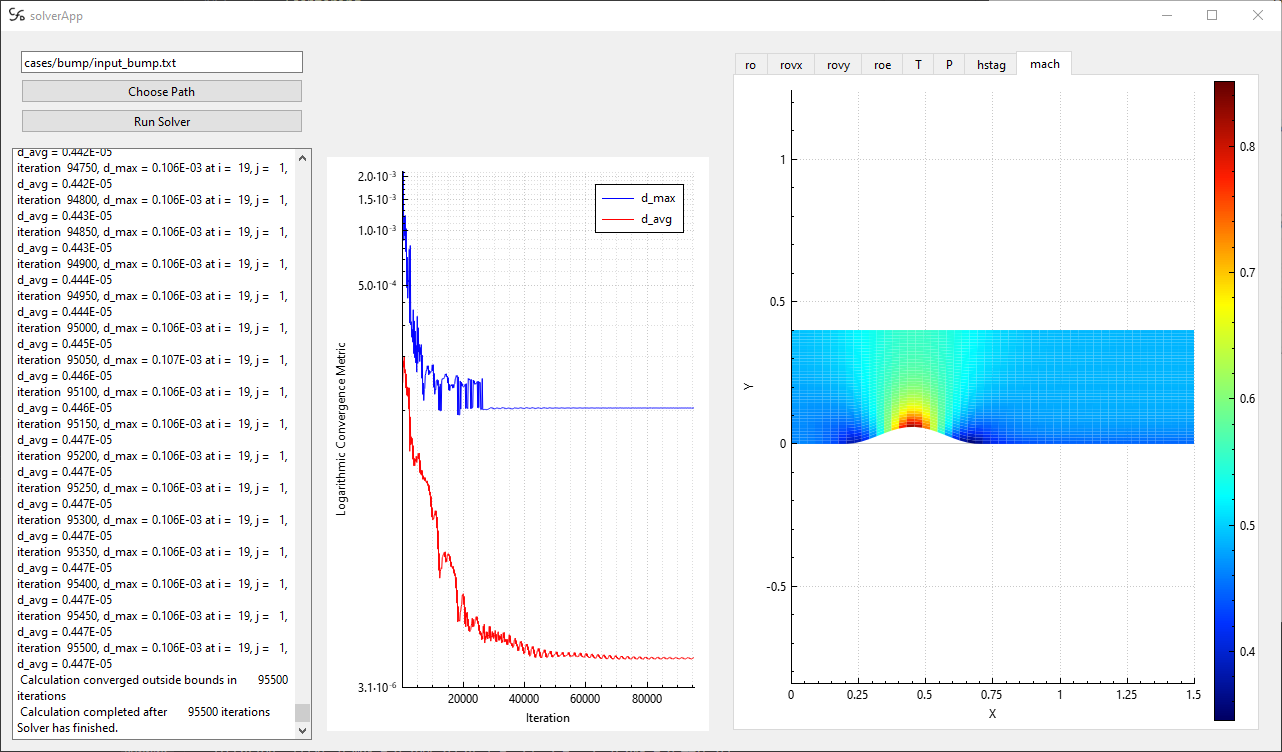
\includegraphics[width=0.8\textwidth]{figures/software.png}
    \caption{The user interface of the software.}
    \label{fig:ui}
\end{figure}

\subsection{Bump test case}

\begin{figure}[H]
    \centering
    \begin{subfigure}{0.99\textwidth}
        \centering
        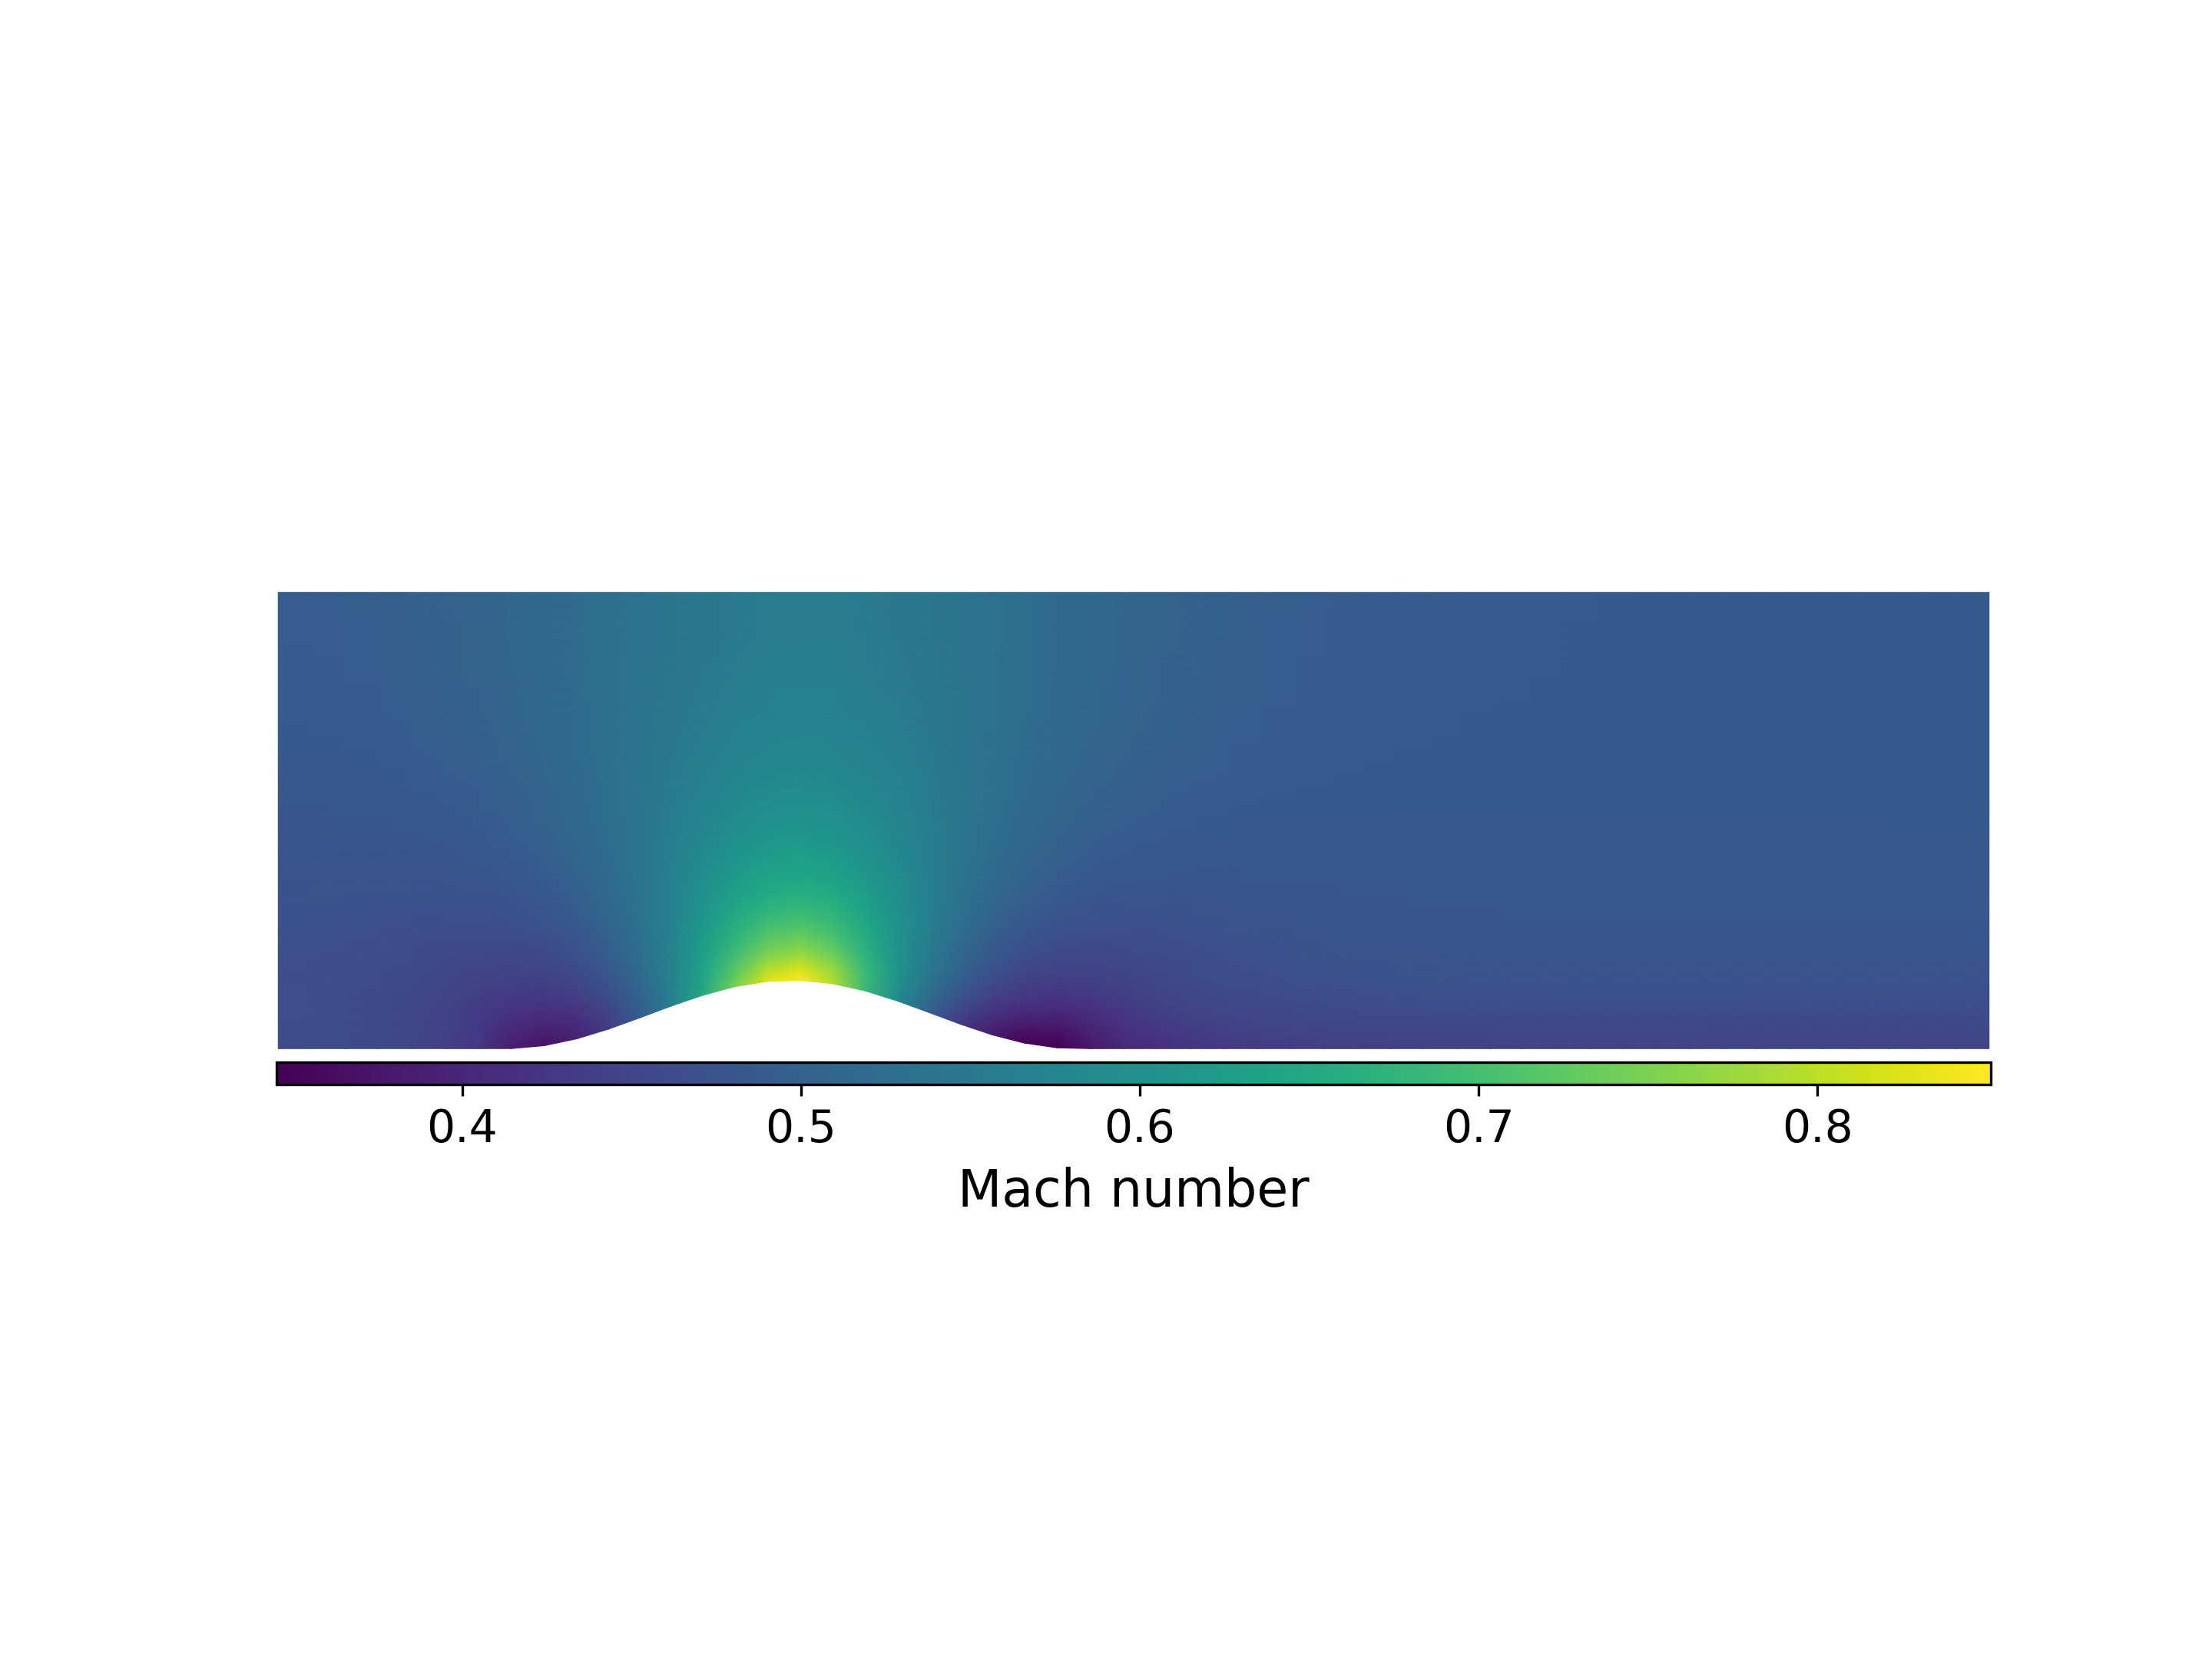
\includegraphics[width=0.7\textwidth]{figures/bump_mach.png}
        \caption{}
        \label{fig:bump_mach}
    \end{subfigure}
    \begin{subfigure}{0.99\textwidth}
        \centering
        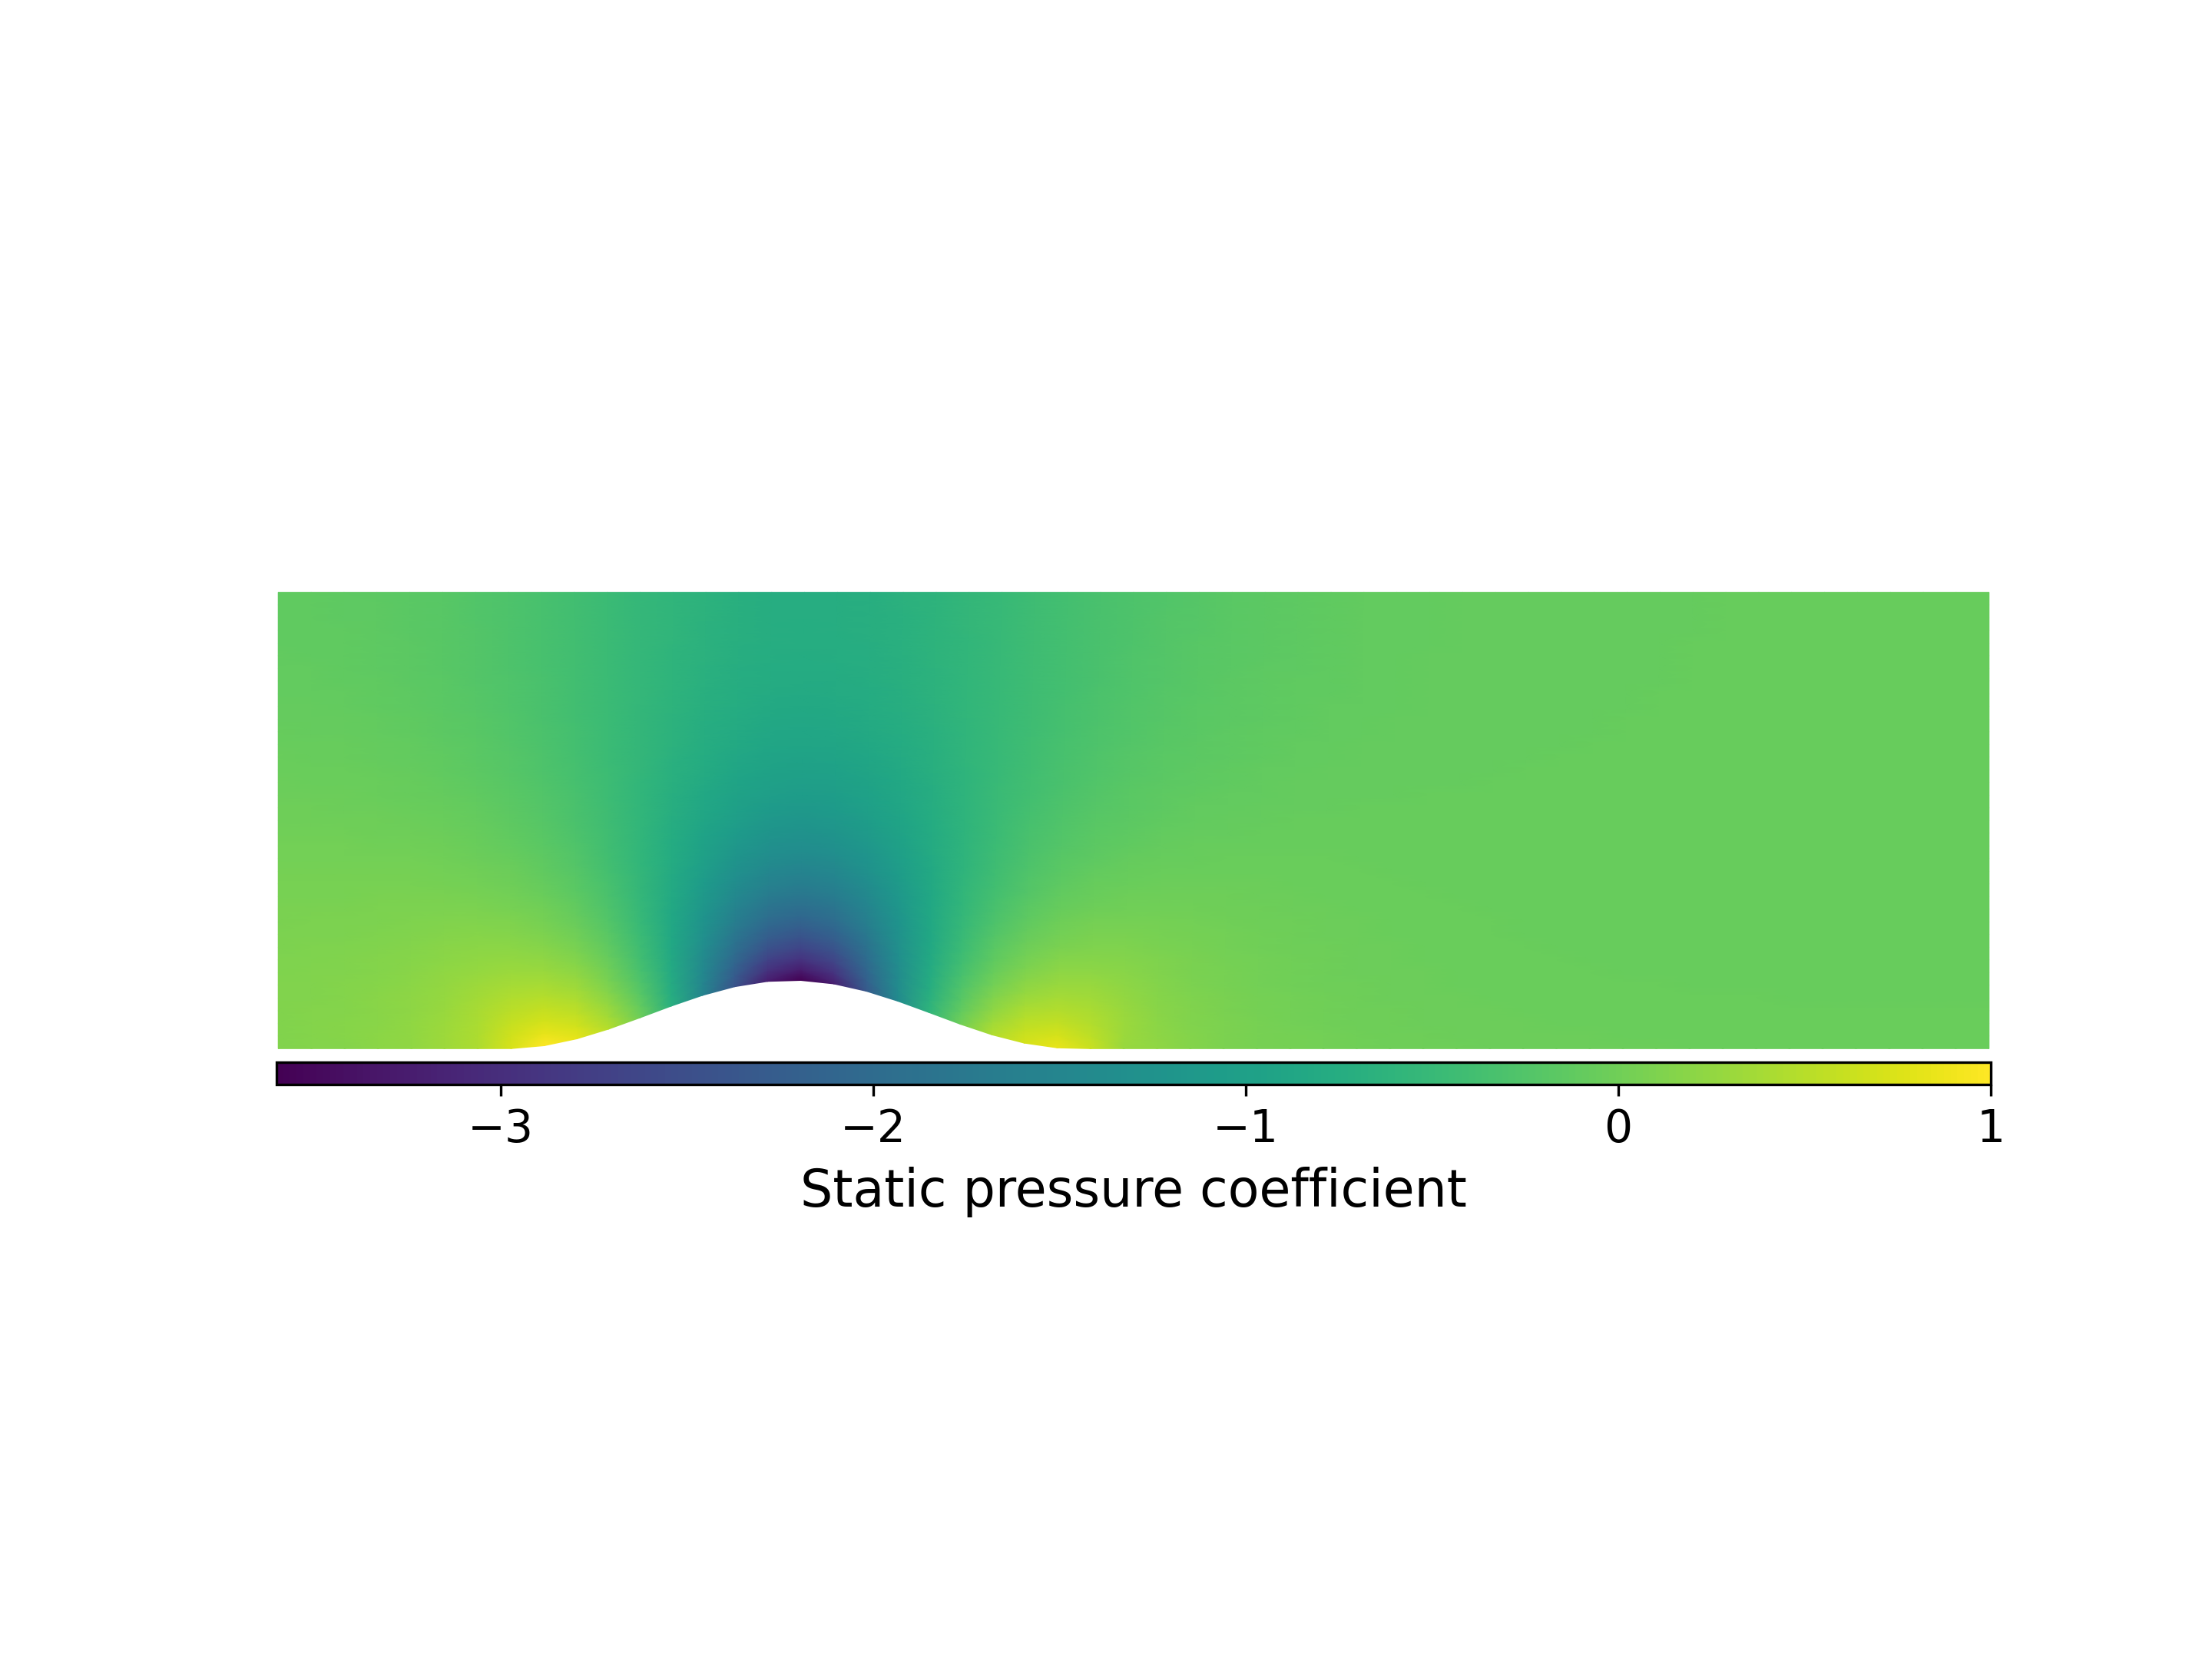
\includegraphics[width=0.7\textwidth]{figures/bump_cp.png}
        \caption{}
        \label{fig:bump_cp}
    \end{subfigure}
    \caption{Bump test case results $CFL = 0.05$, $sfac = 0.1$, $n_i = 53$, $n_j = 37$.}
\end{figure}

\begin{figure}[H]
    \centering
    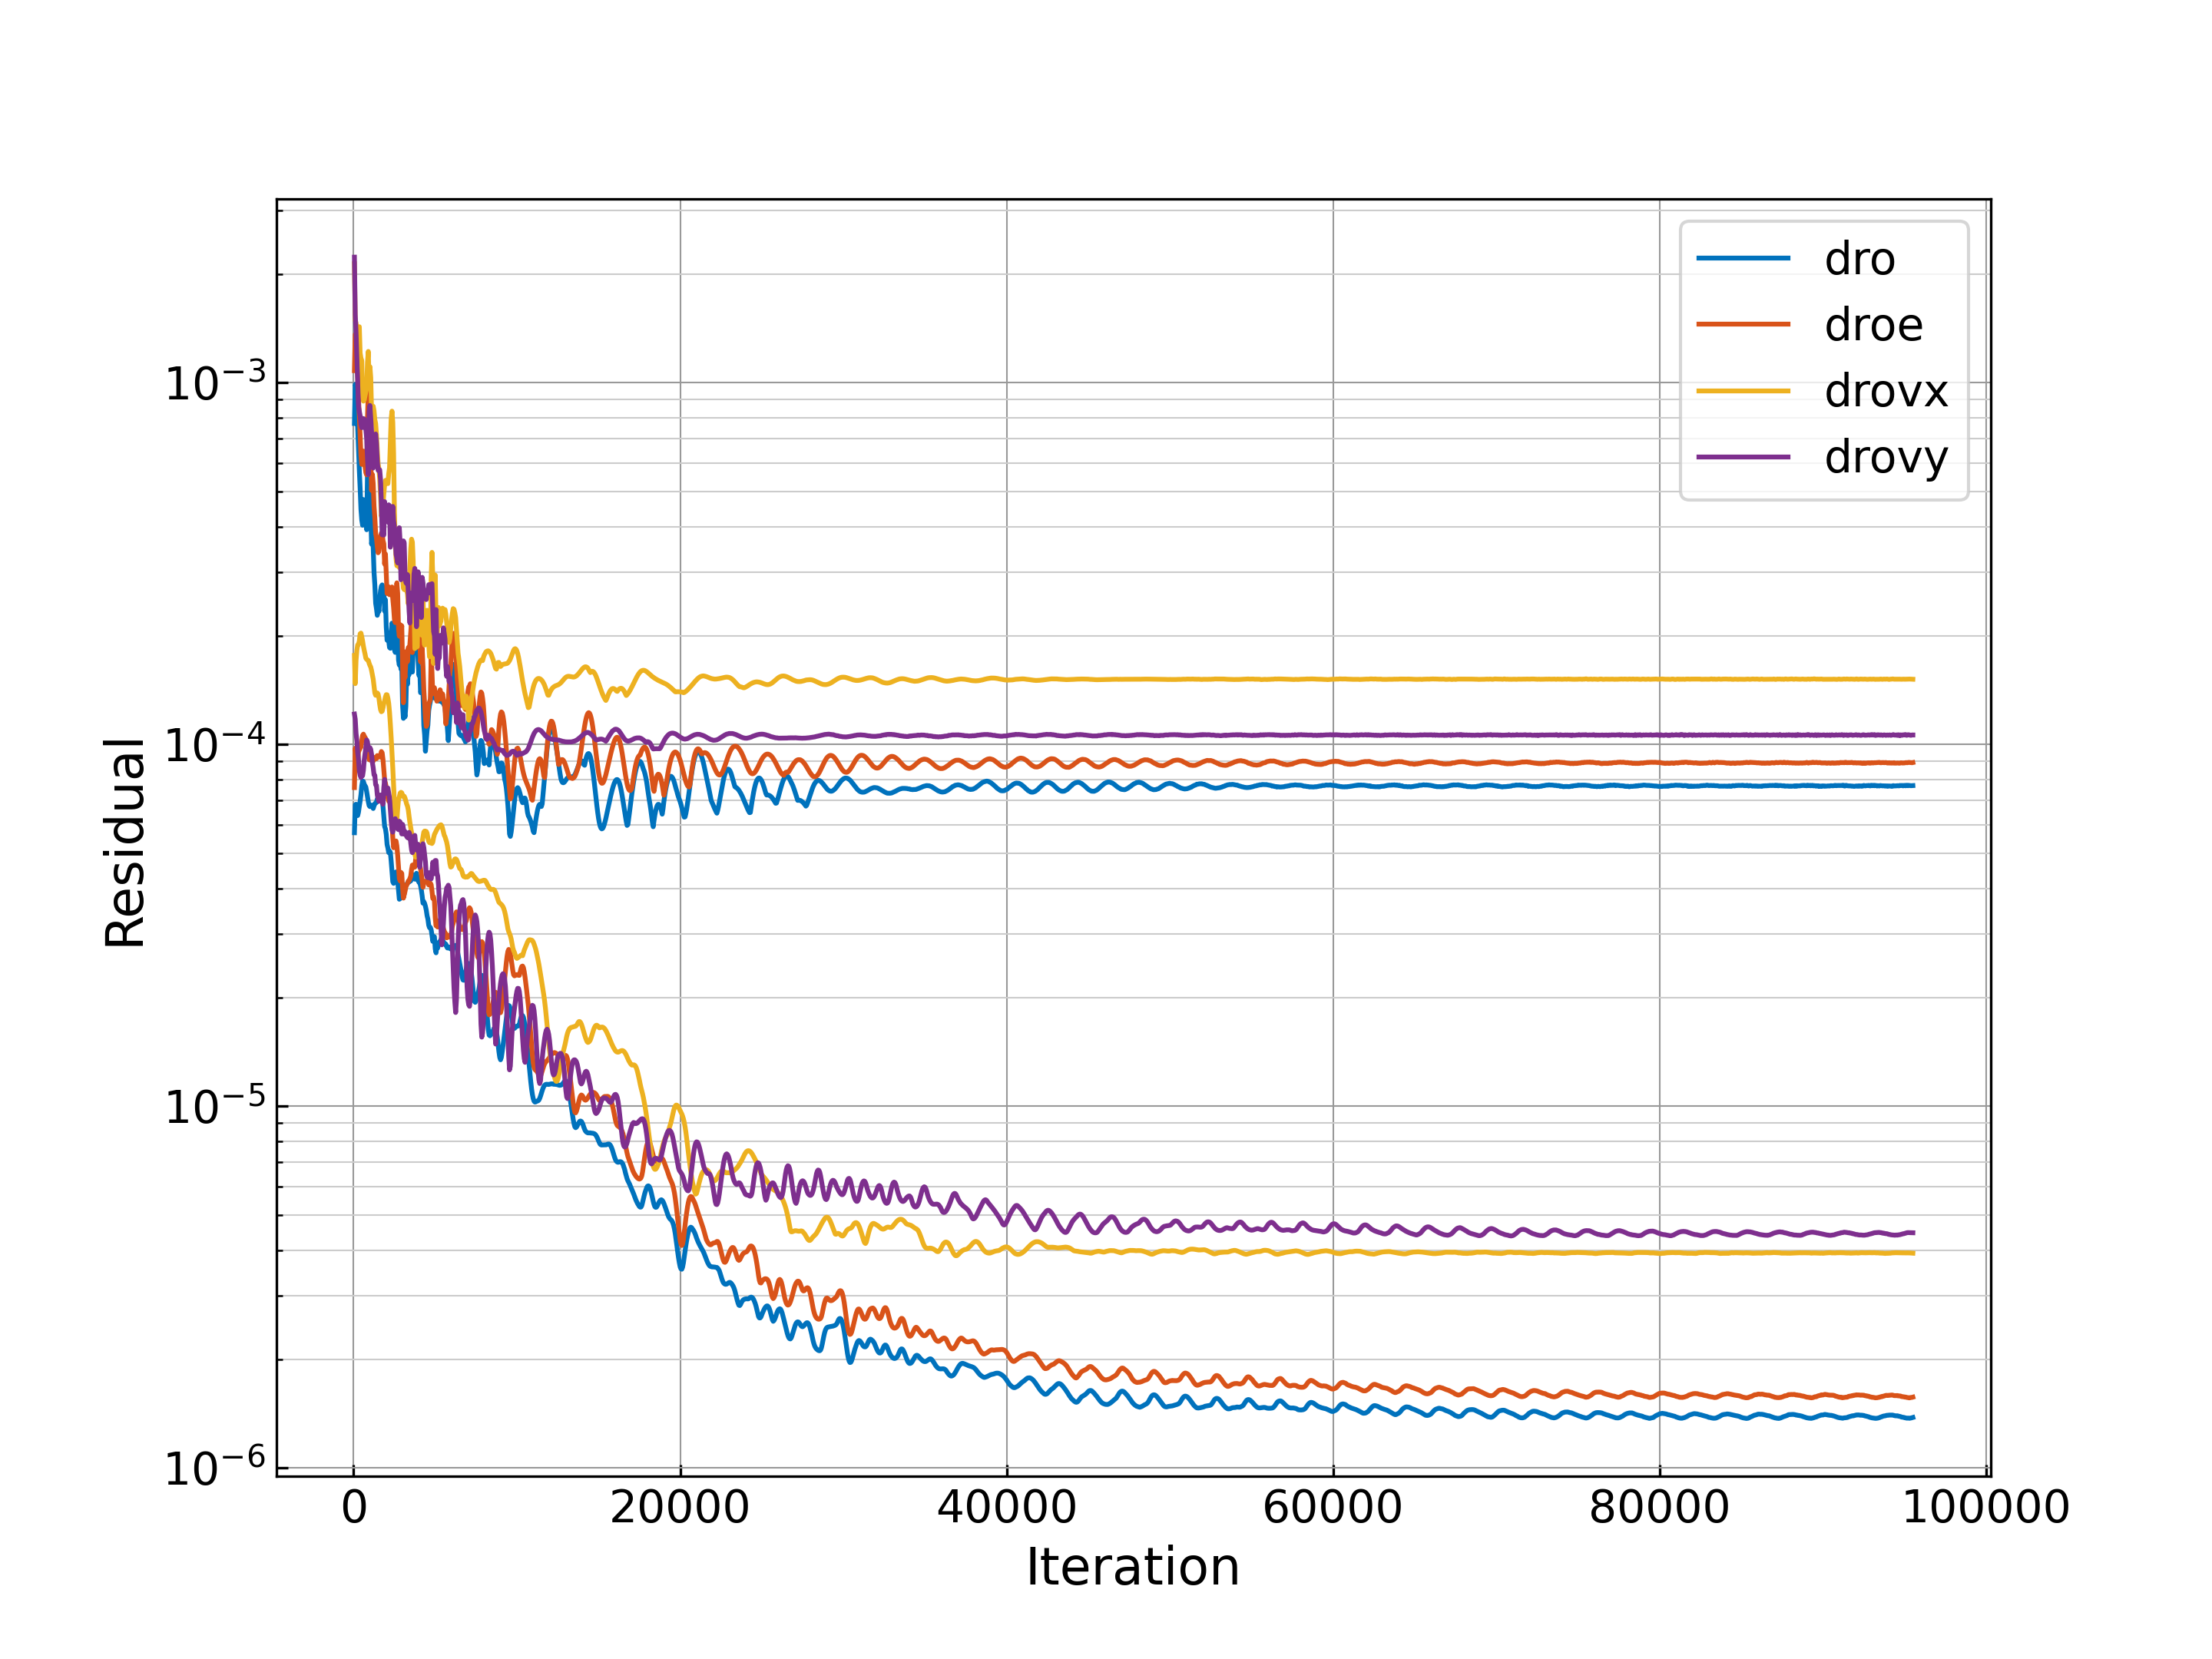
\includegraphics[width=0.7\textwidth]{figures/bump_conv.png}
    \caption{Convergence history of primary flow variables for the bump case}
    \label{fig:bump_conv}
\end{figure}

\begin{figure}[H]
    \centering
    \begin{subfigure}{0.49\textwidth}
        \centering
        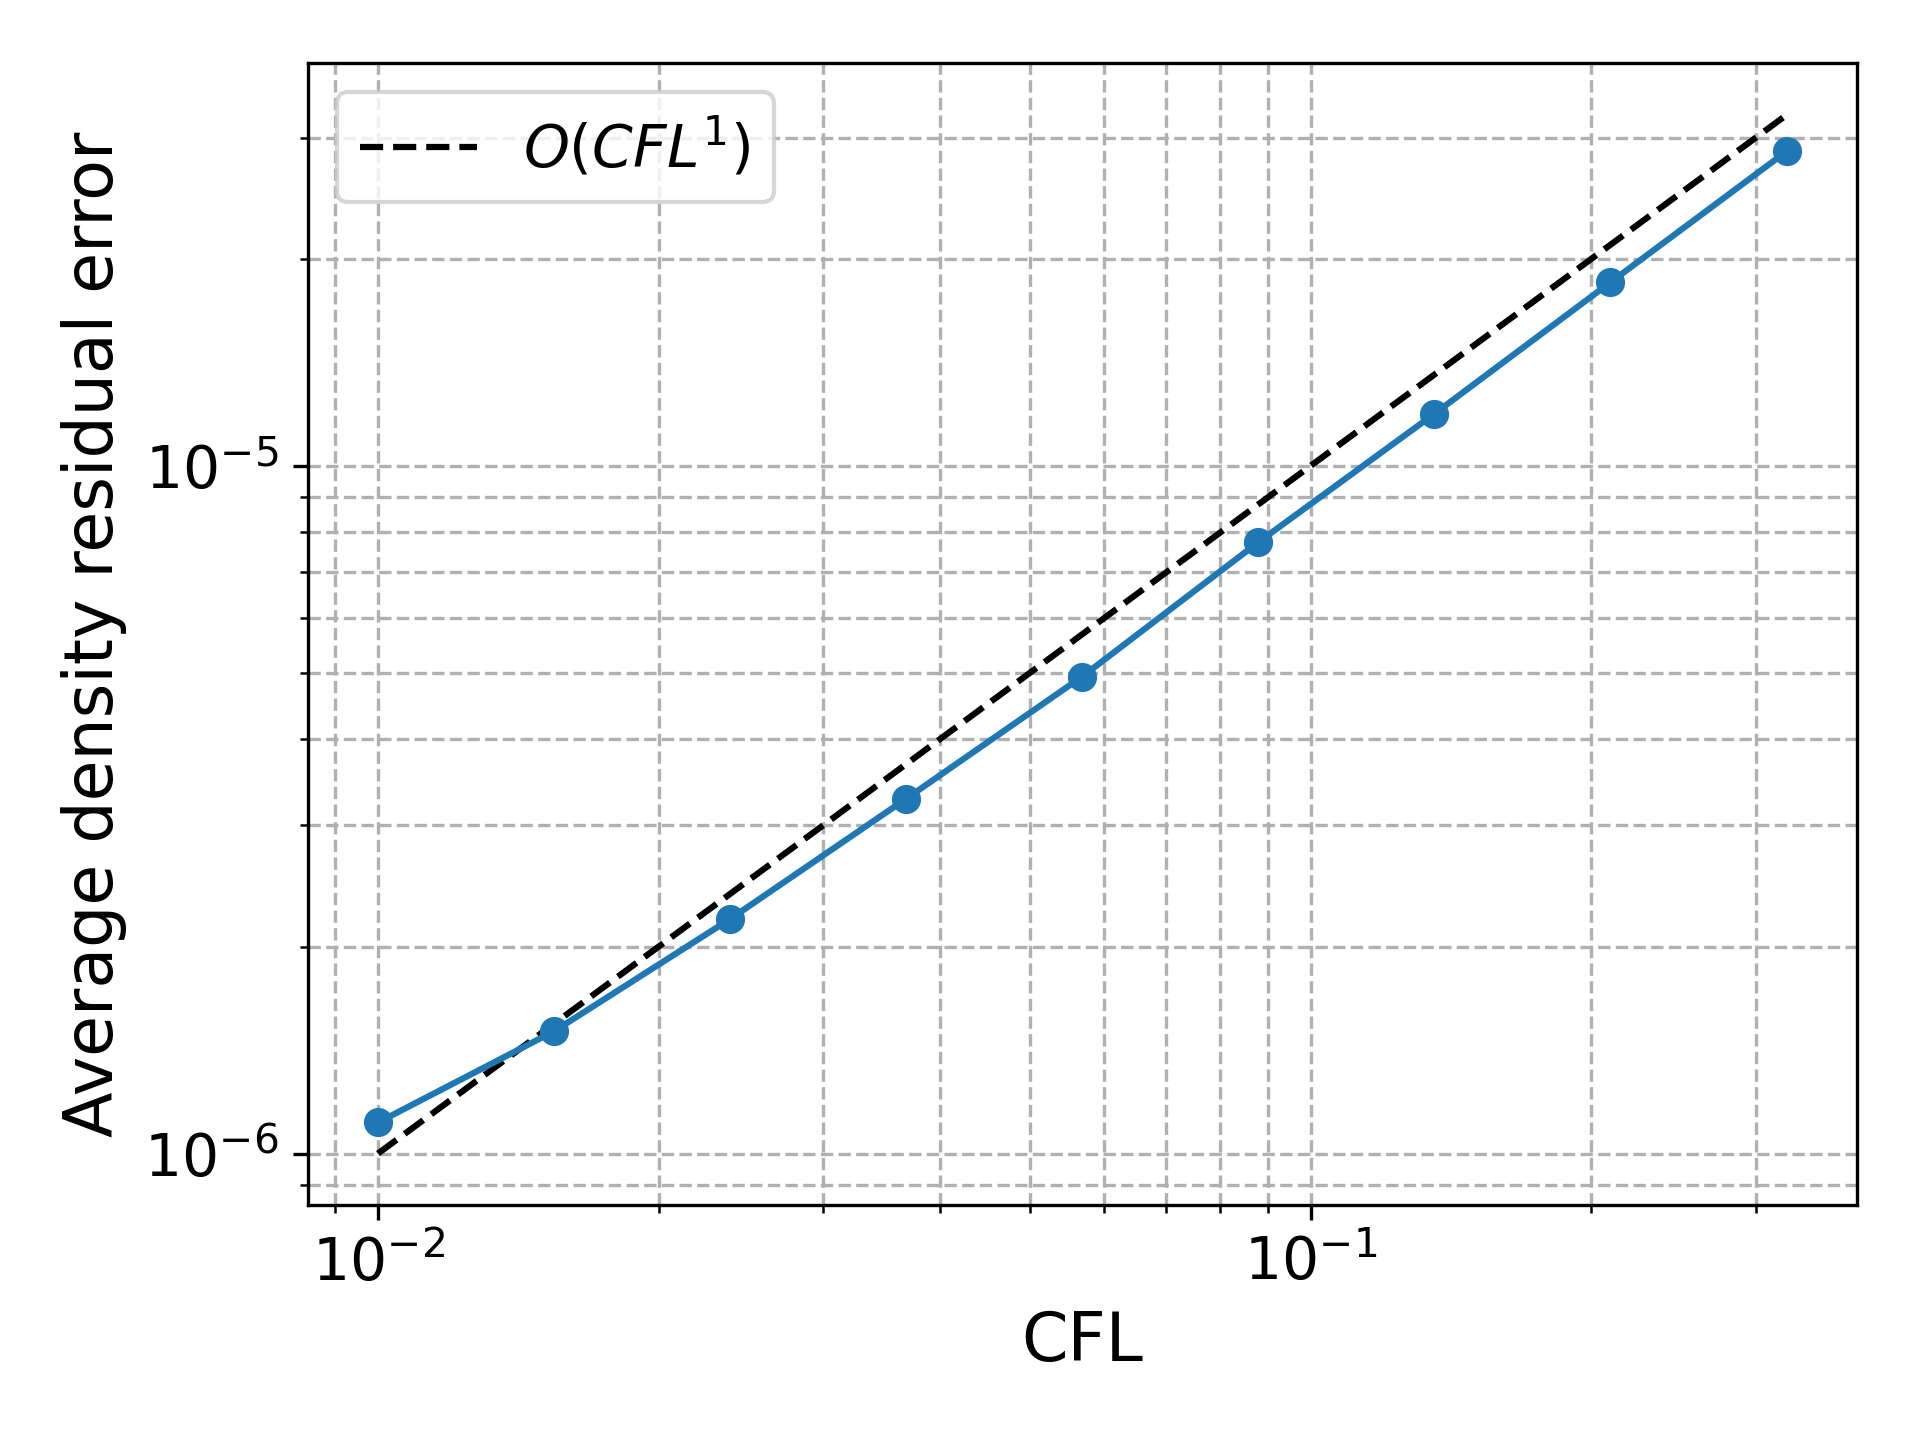
\includegraphics[width=0.99\textwidth]{figures/bump_d_avg_cfl.png}
        \caption{}
        \label{fig:bump_d_avg_cfl}
    \end{subfigure}
    \begin{subfigure}{0.49\textwidth}
        \centering
        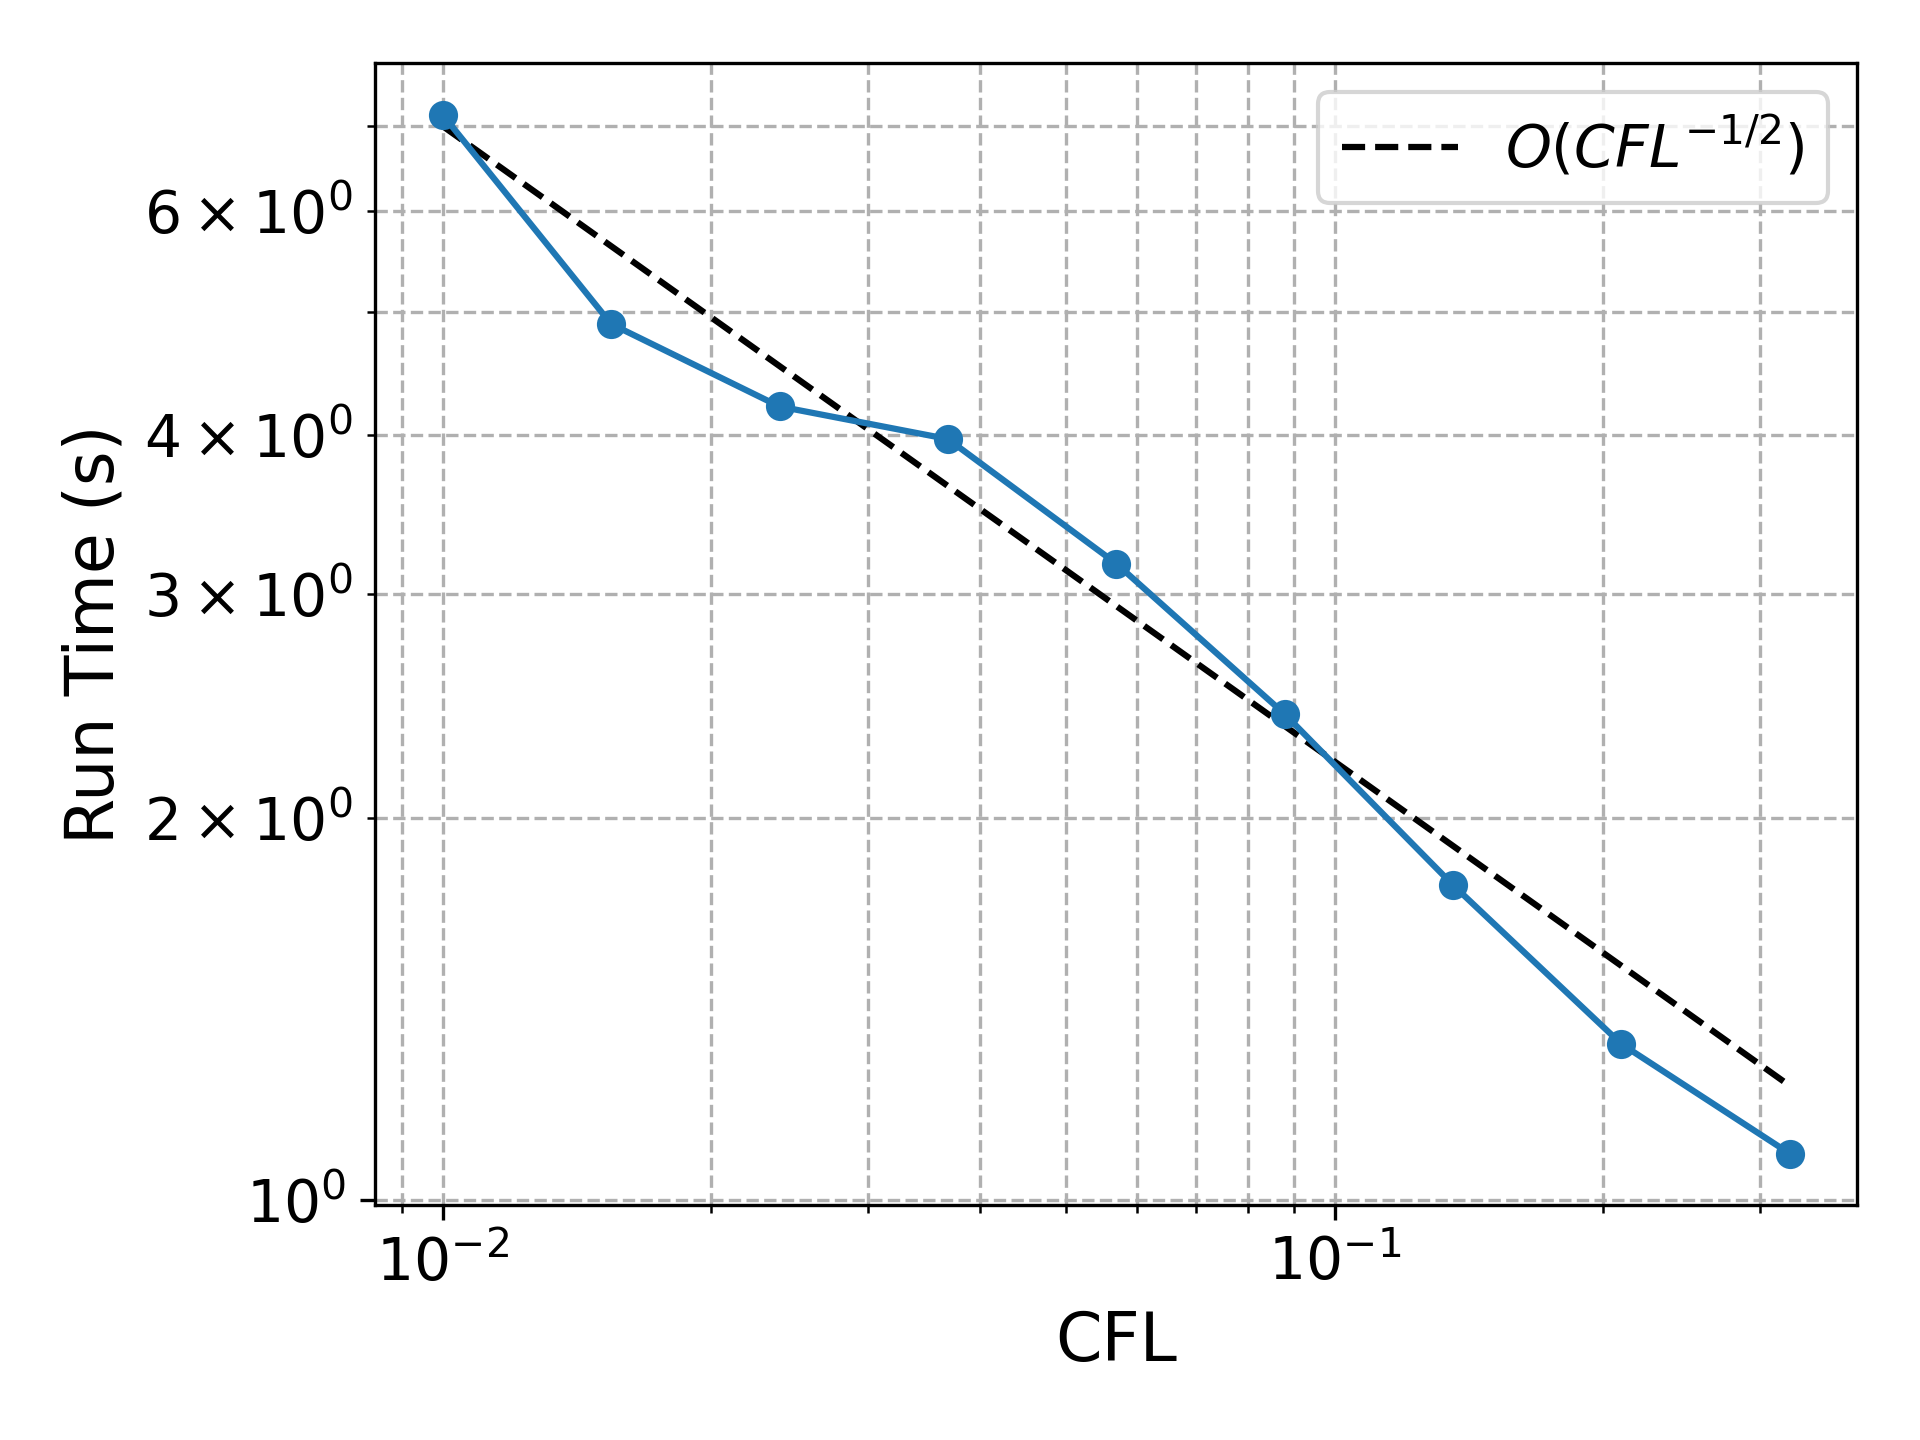
\includegraphics[width=0.99\textwidth]{figures/bump_time_cfl.png}
        \caption{}
        \label{fig:bump_time_cfl}
    \end{subfigure}
    
    \caption{Average density residual and run time against $CFL$ for the bump case where $sfac = 0.5$, $ni = 53$.}
\end{figure}

\begin{figure}[H]
    \centering
    \begin{subfigure}{0.49\textwidth}
        \centering
        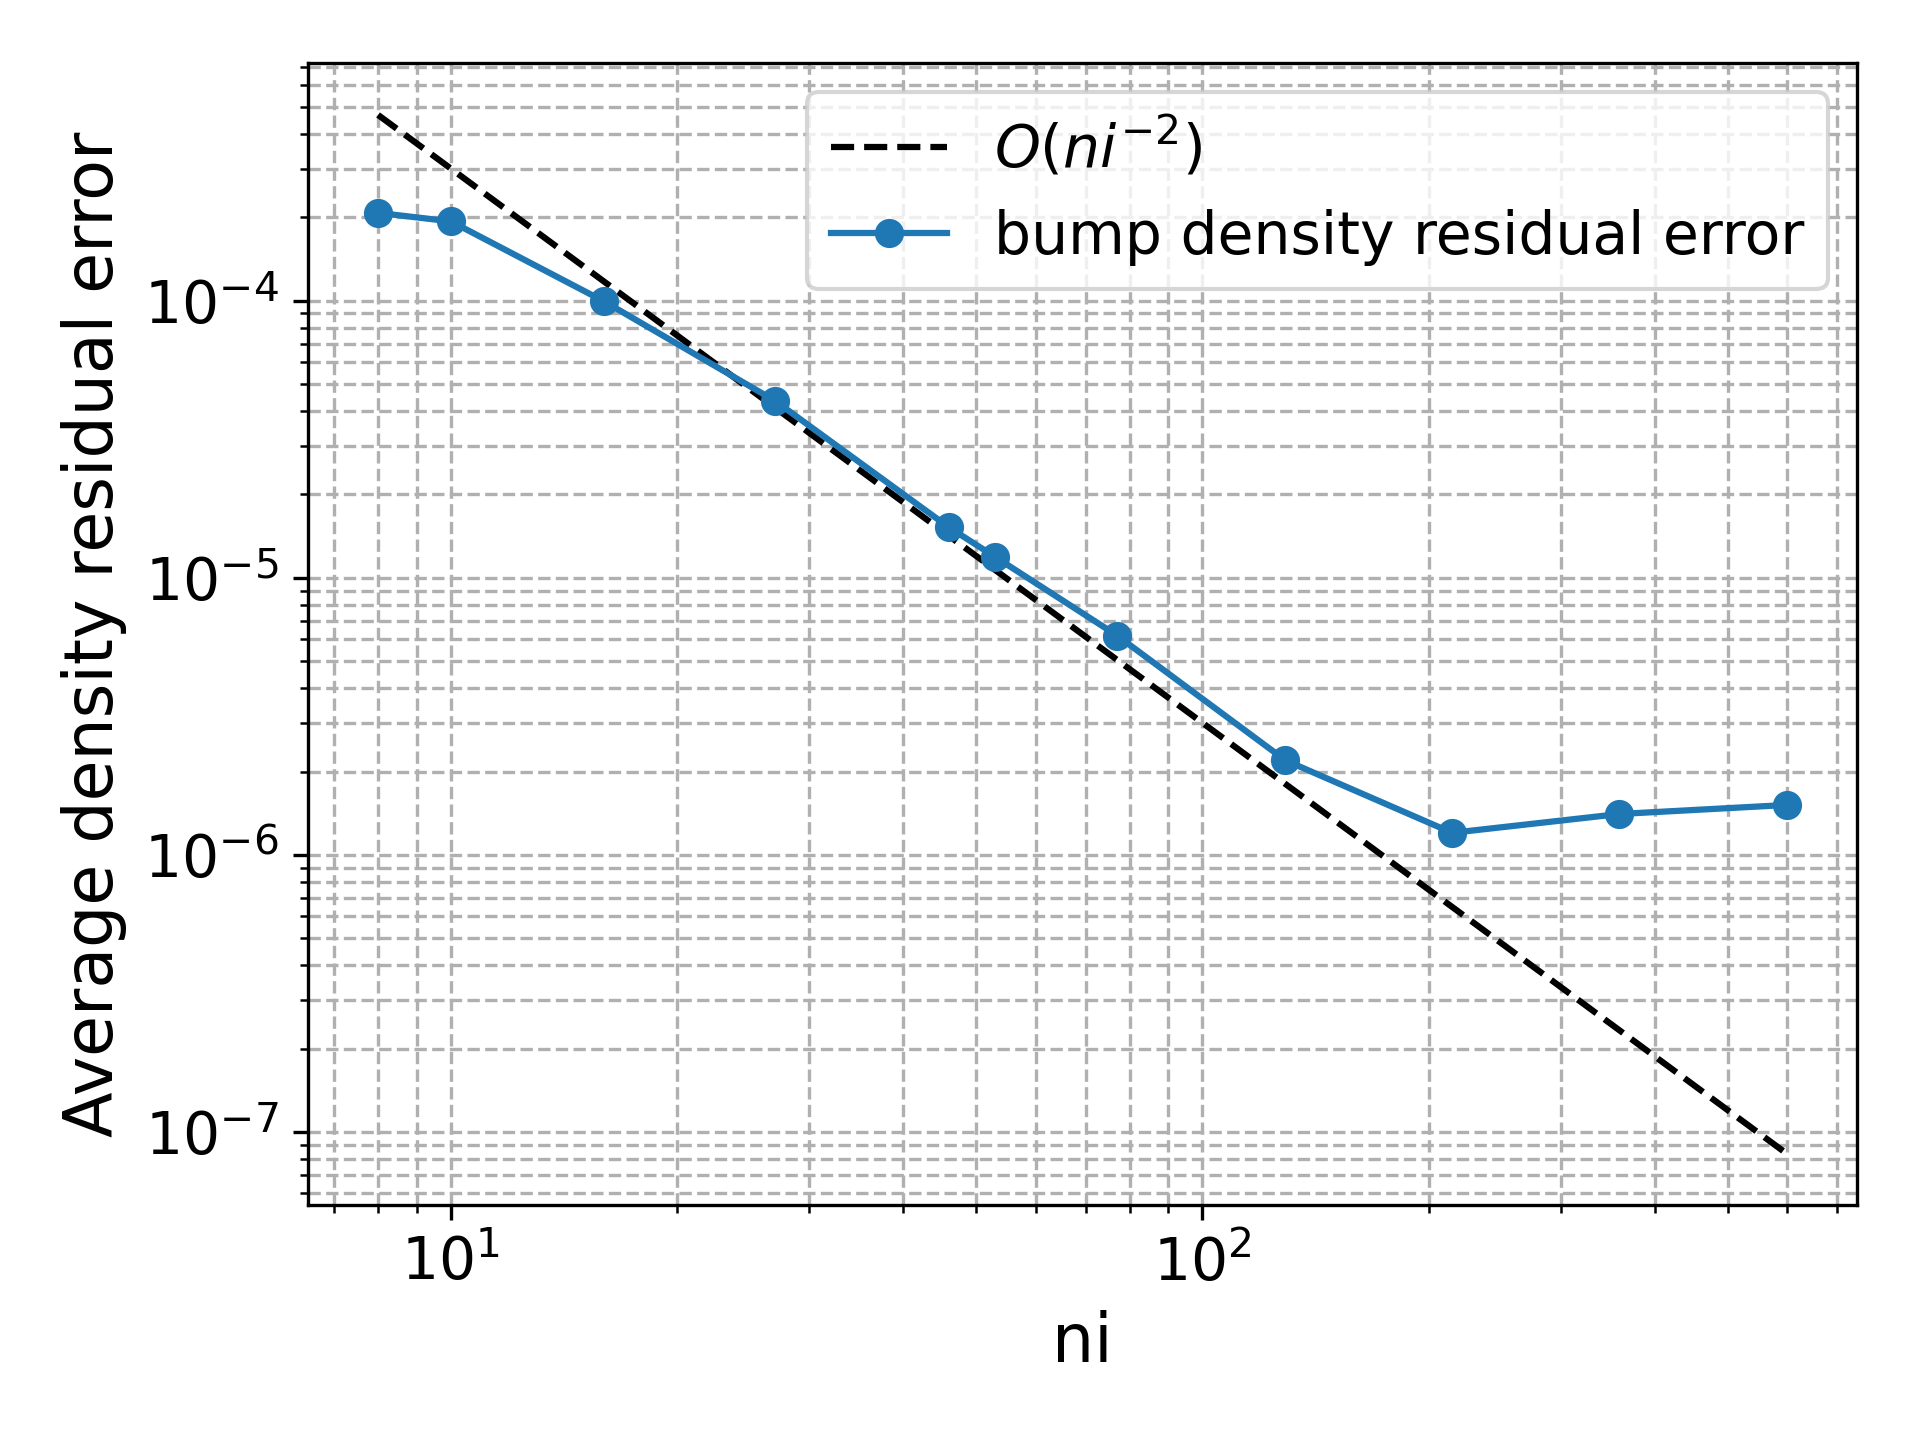
\includegraphics[width=0.99\textwidth]{figures/bump_d_avg_ni.png}
        \caption{}
        \label{fig:bump_d_avg_ni}
    \end{subfigure}
    \begin{subfigure}{0.49\textwidth}
        \centering
        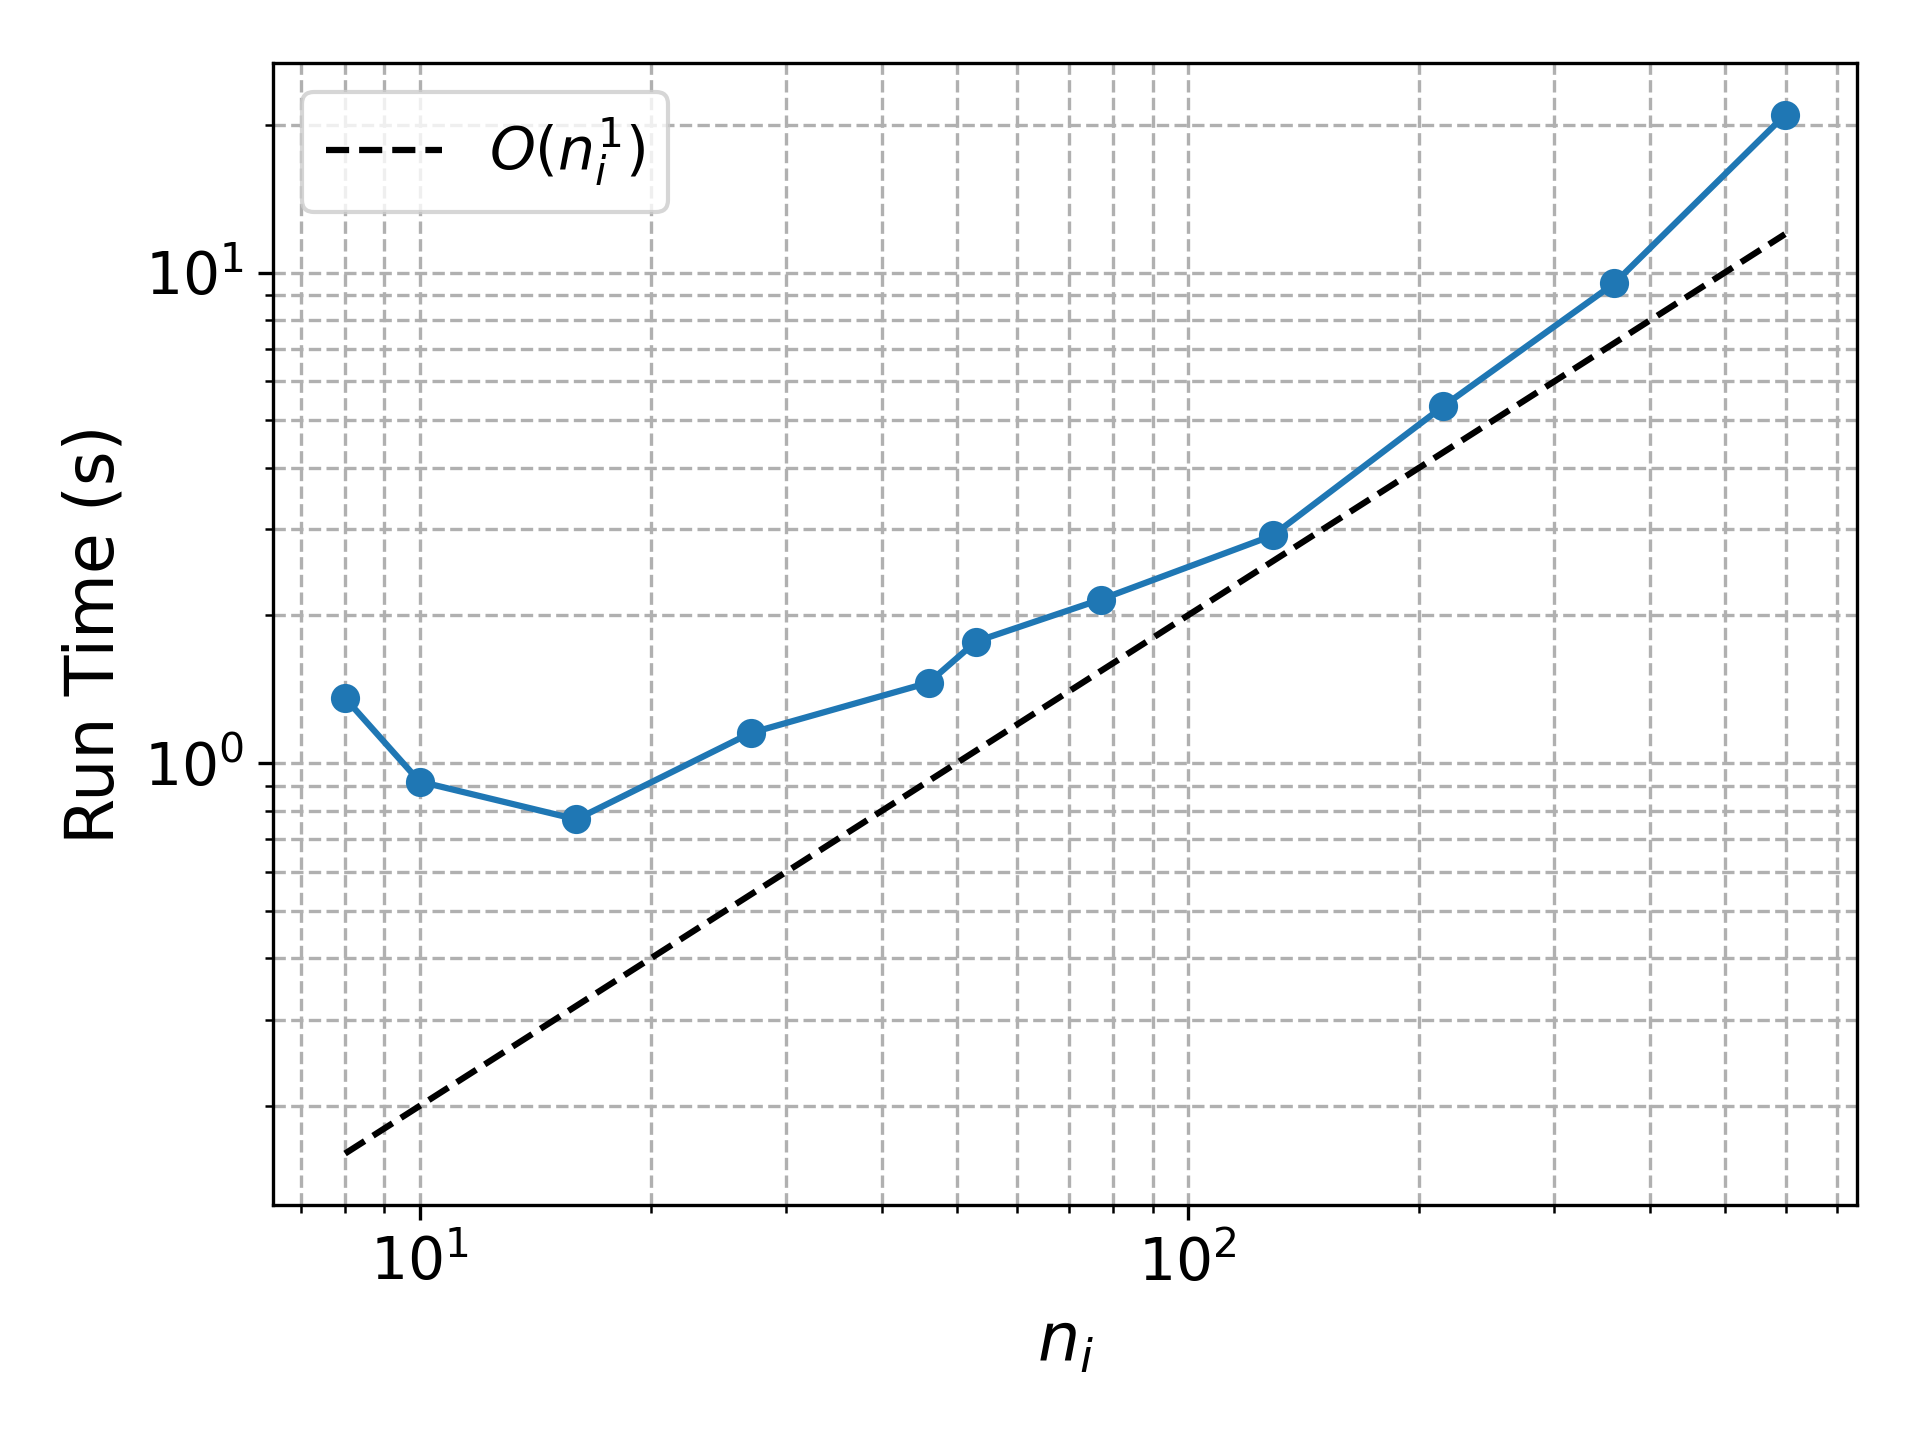
\includegraphics[width=0.99\textwidth]{figures/bump_time_ni.png}
        \caption{}
        \label{fig:bump_time_ni}
    \end{subfigure}
    \caption{Average density residual and run time against $n_i$ for the bump case where $sfac = 0.5$, $sfac = 0.1357$.}
\end{figure}

\begin{figure}[H]
    \centering
    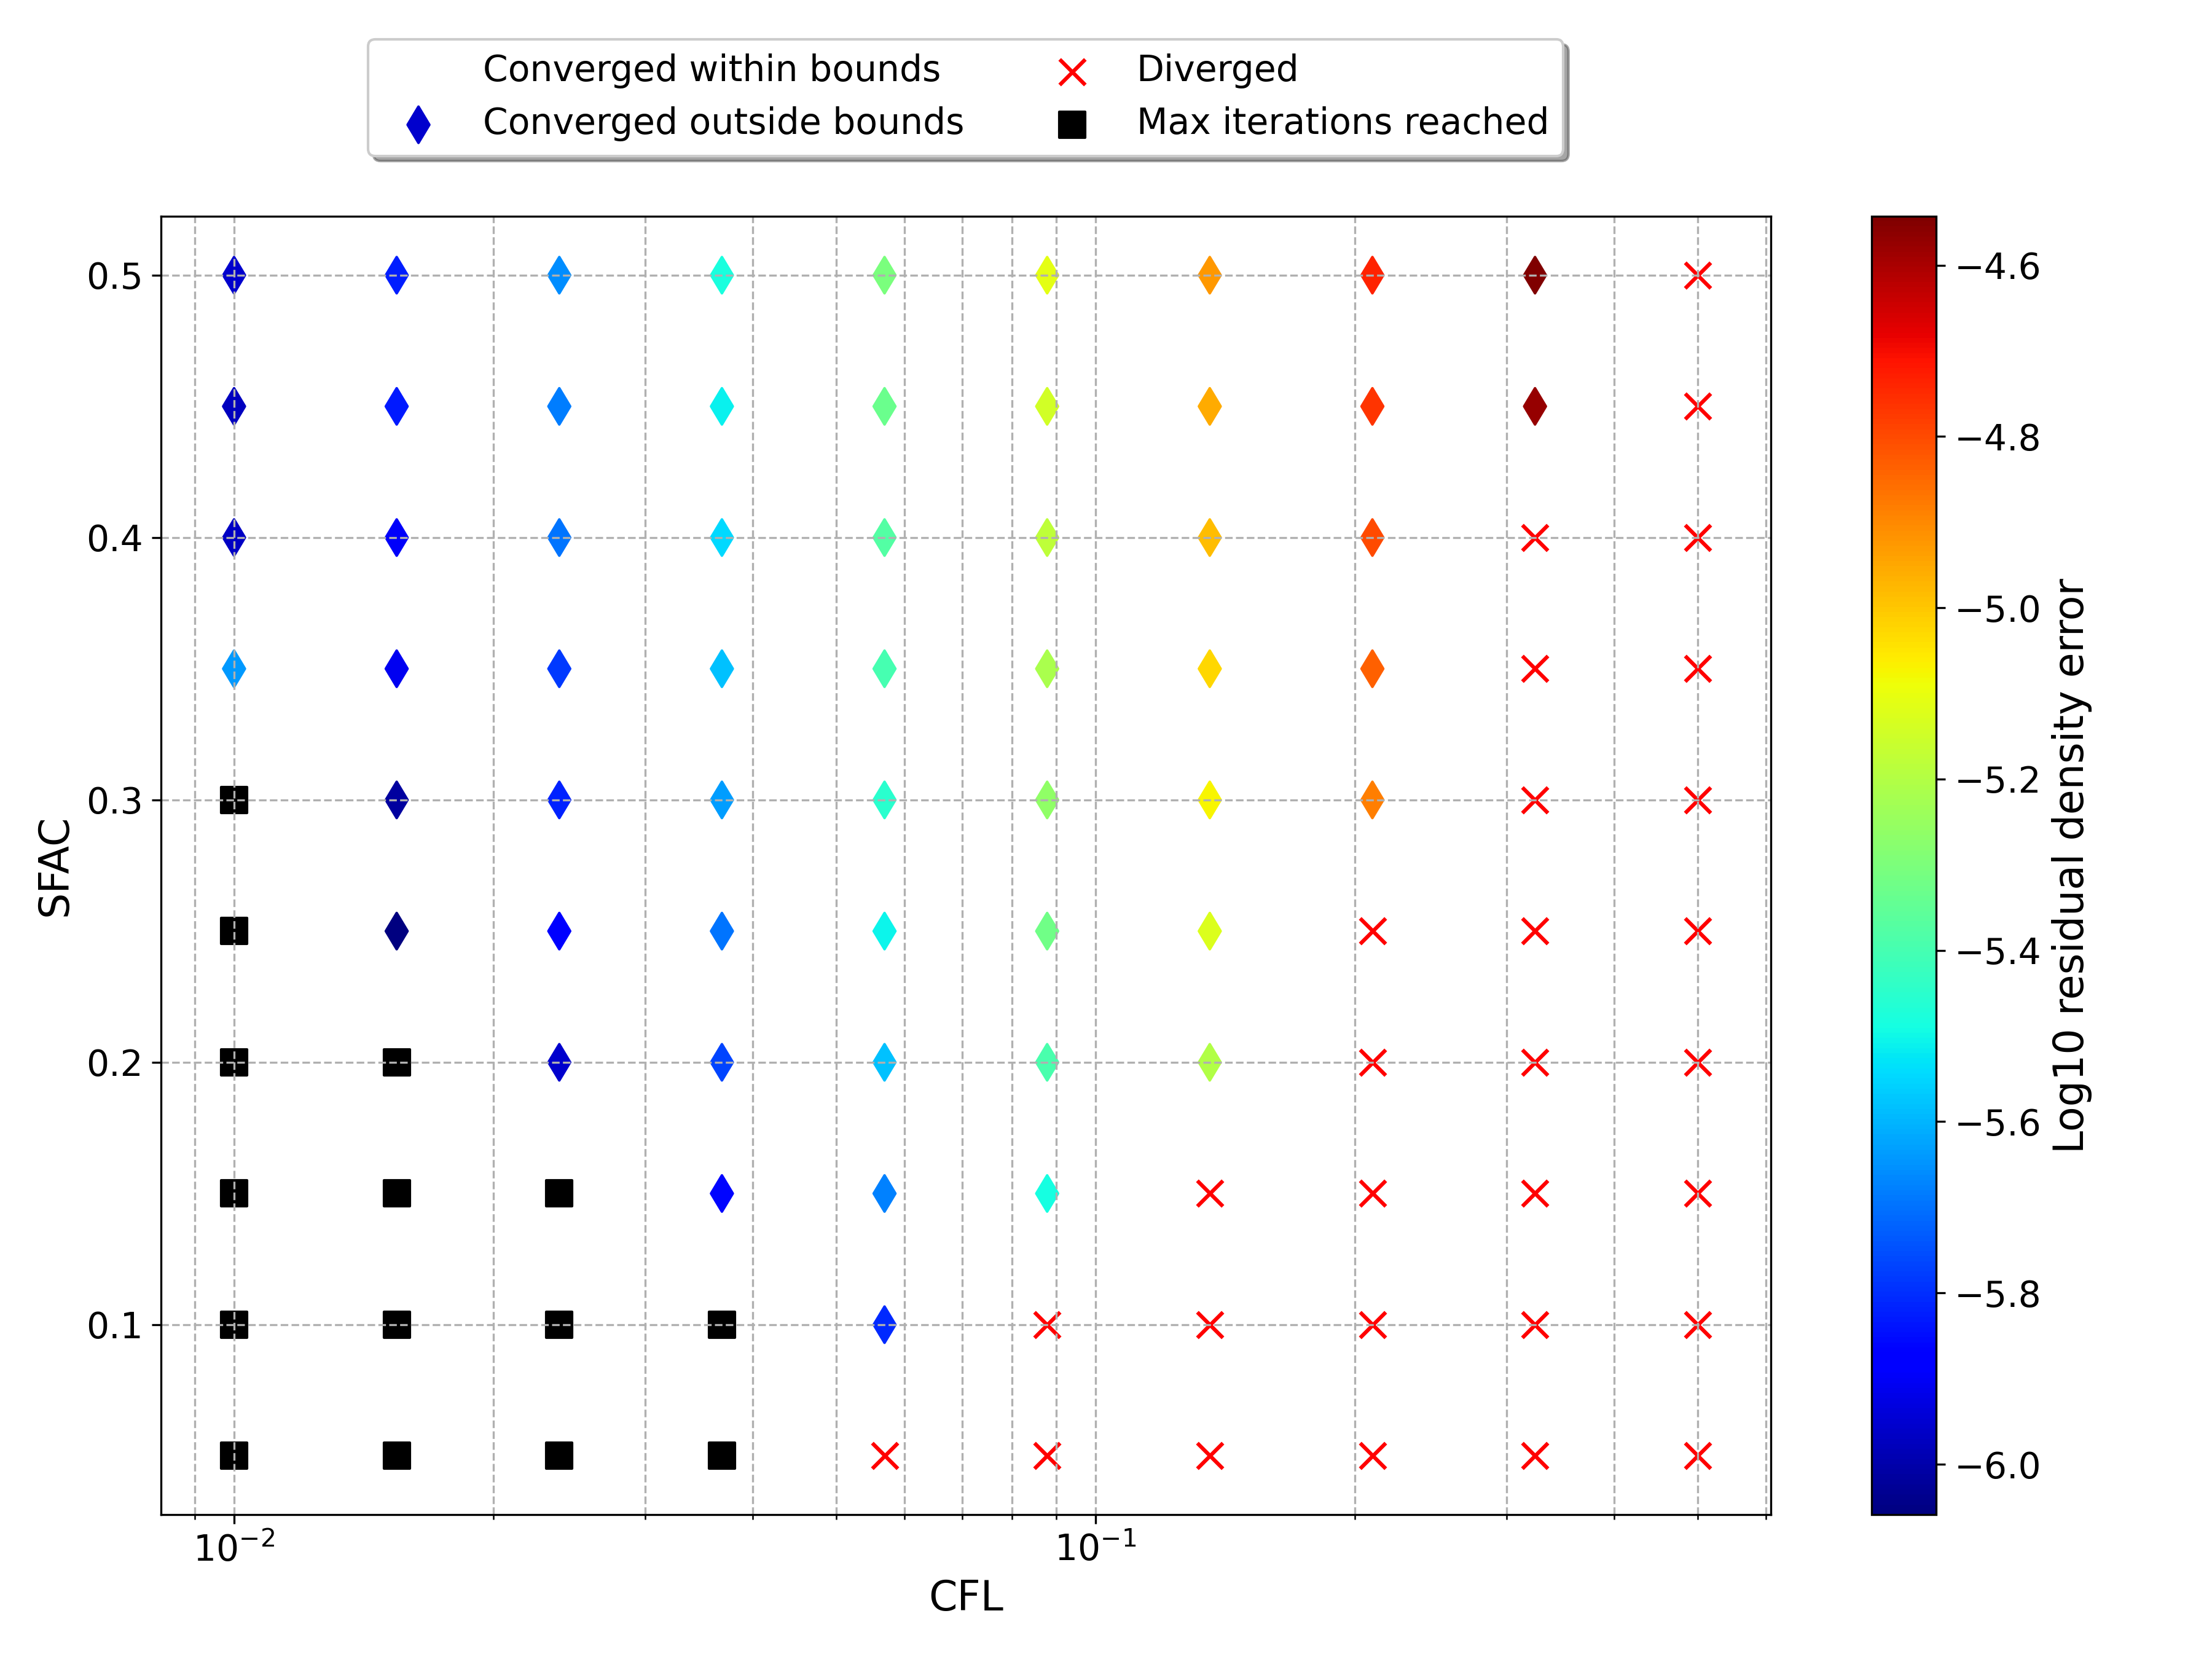
\includegraphics[width=0.8\textwidth]{figures/bump_cfl_sfac_residual.png}
    \caption{Scatter plot showing variation in residual error for different CFL and sfac values.}
    \label{fig:bump_cfl_sfac_residual}
\end{figure}

\begin{figure}[H]
    \centering
    \centering
    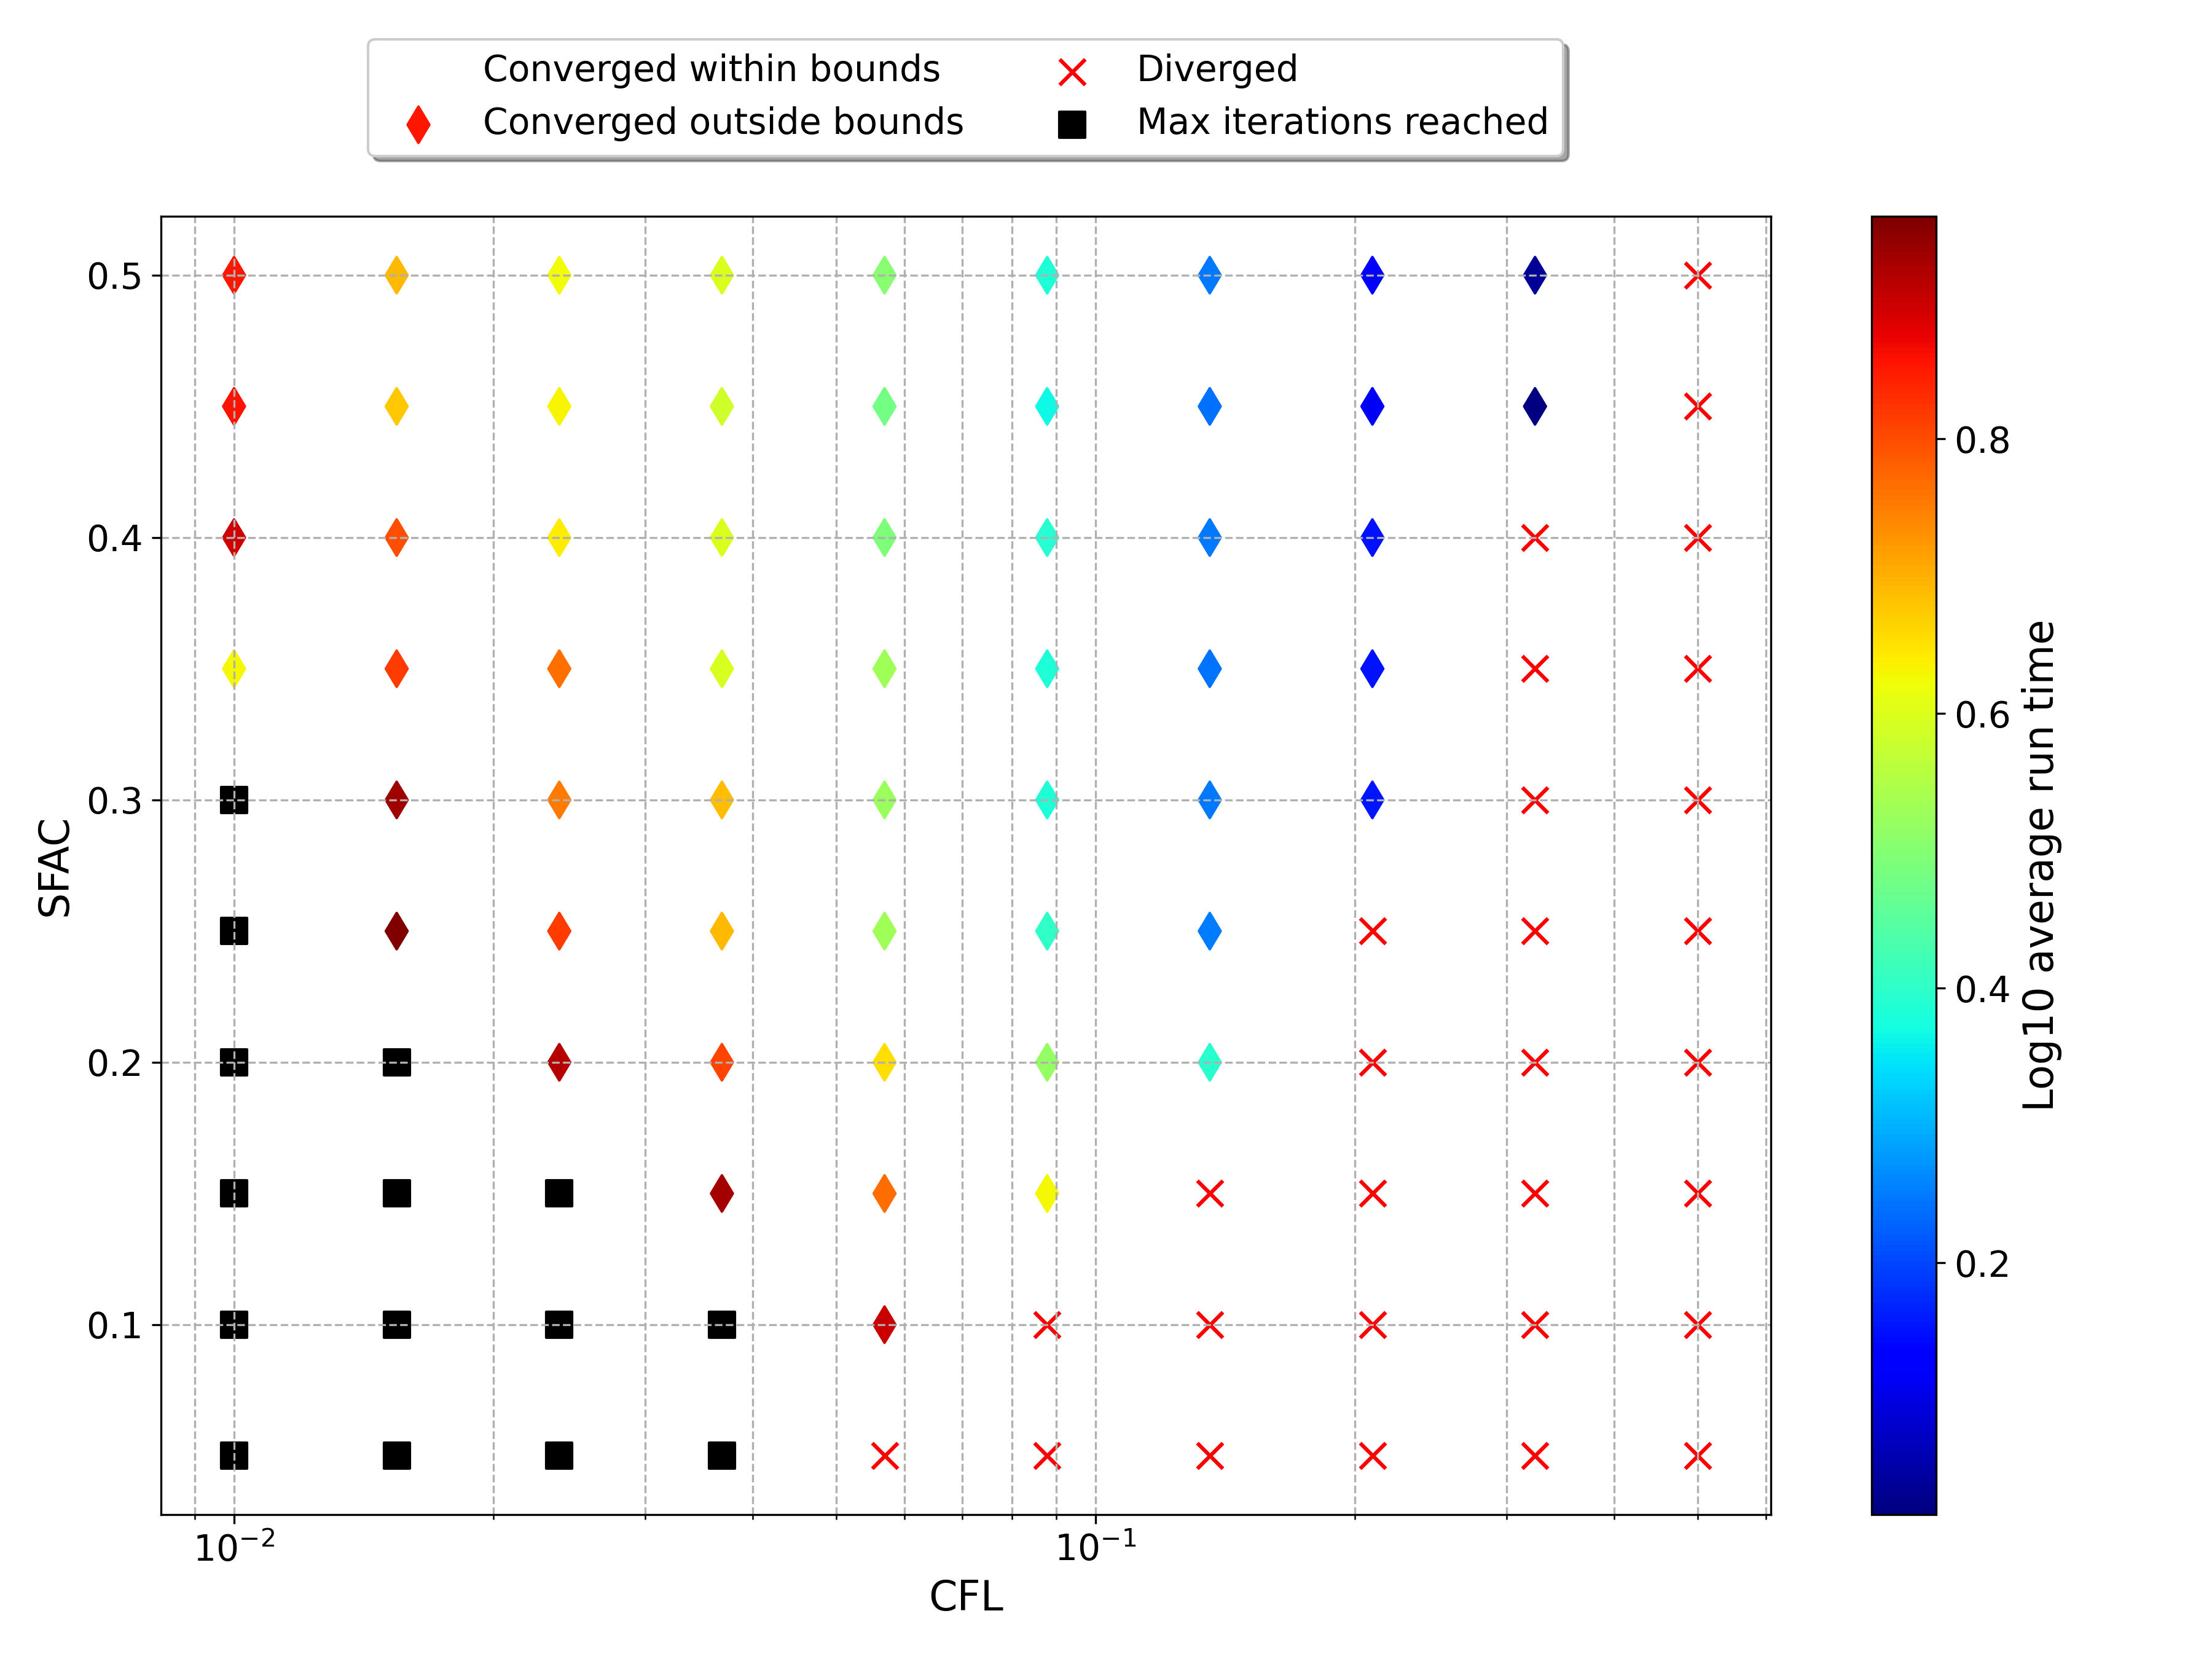
\includegraphics[width=0.8\textwidth]{figures/bump_cfl_sfac_time.png}
    \caption{Scatter plot showing variation in run time for different CFL and sfac values.}
    \label{fig:bump_cfl_sfac_time}
\end{figure}

\begin{figure}[H]
    \centering
    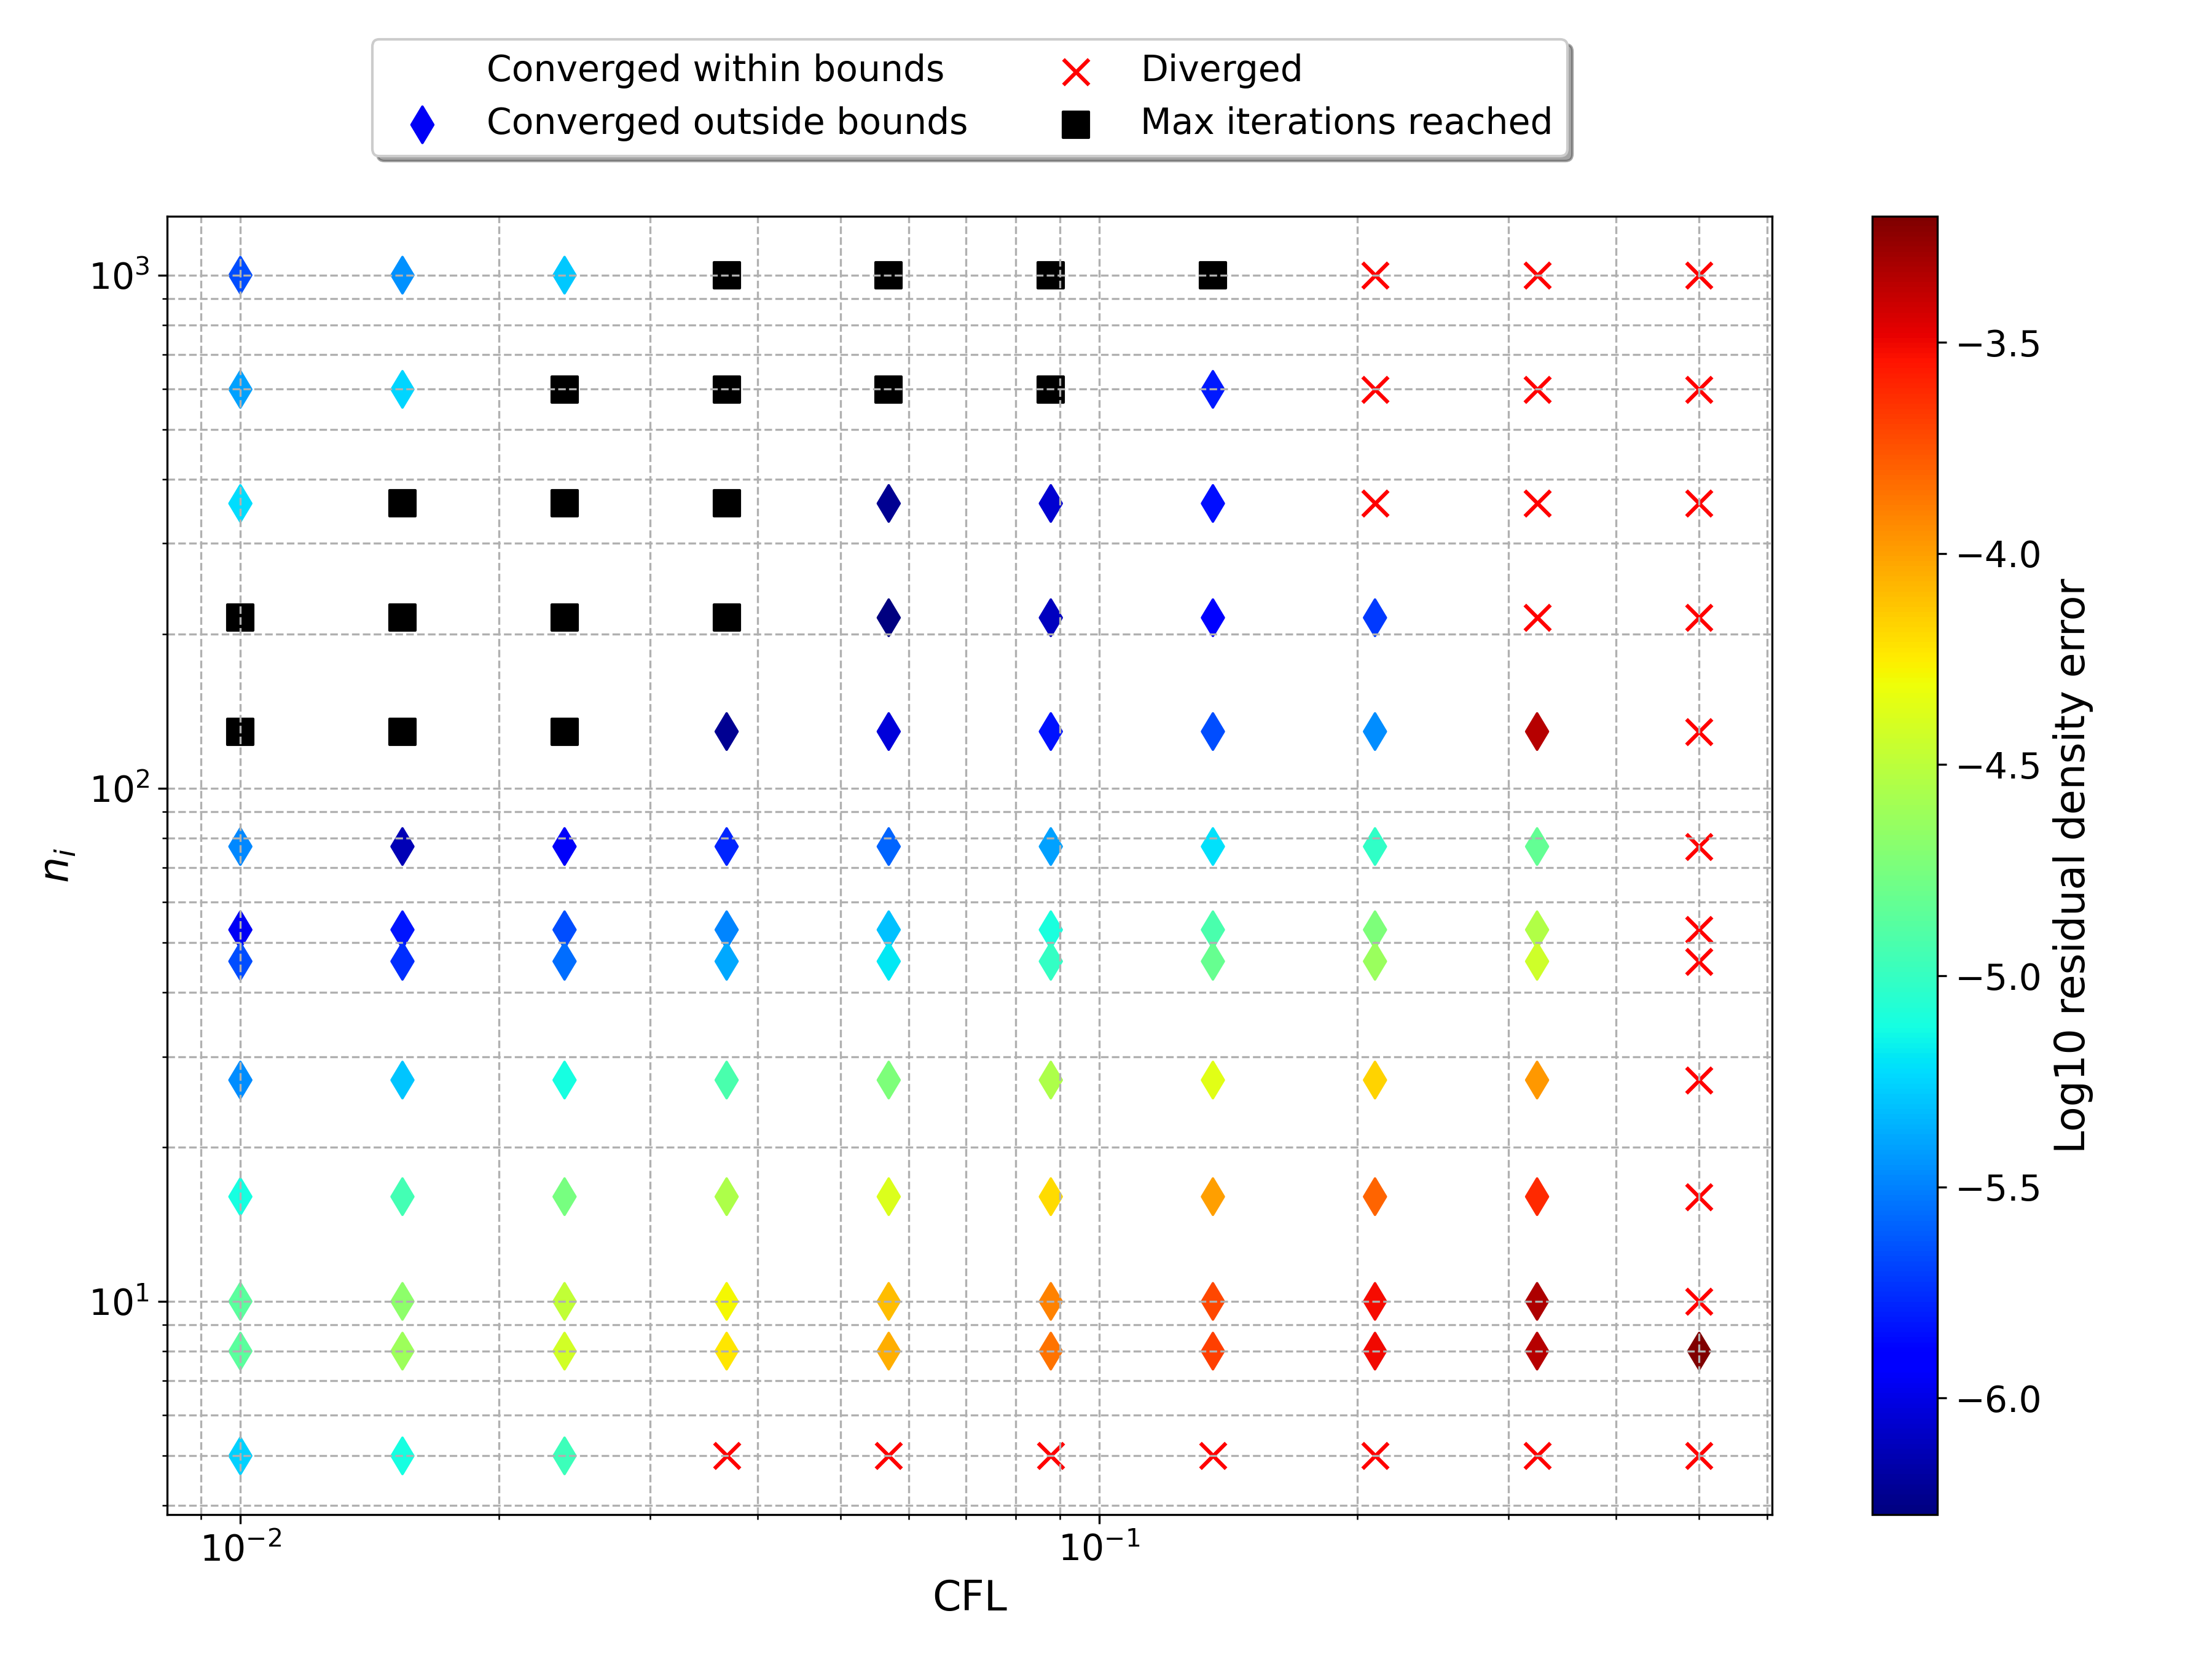
\includegraphics[width=0.8\textwidth]{figures/bump_ni_cfl_residual.png}
    \caption{Scatter plot showing variation in residual error for different $CFL$ and $n_i$ values. $sfac = 0.5$. Runs in the top left are incorrectly marked as converged by the solver.}
    \label{fig:bump_ni_cfl_residual}
\end{figure}

\begin{figure}[H]
    \centering
    \centering
    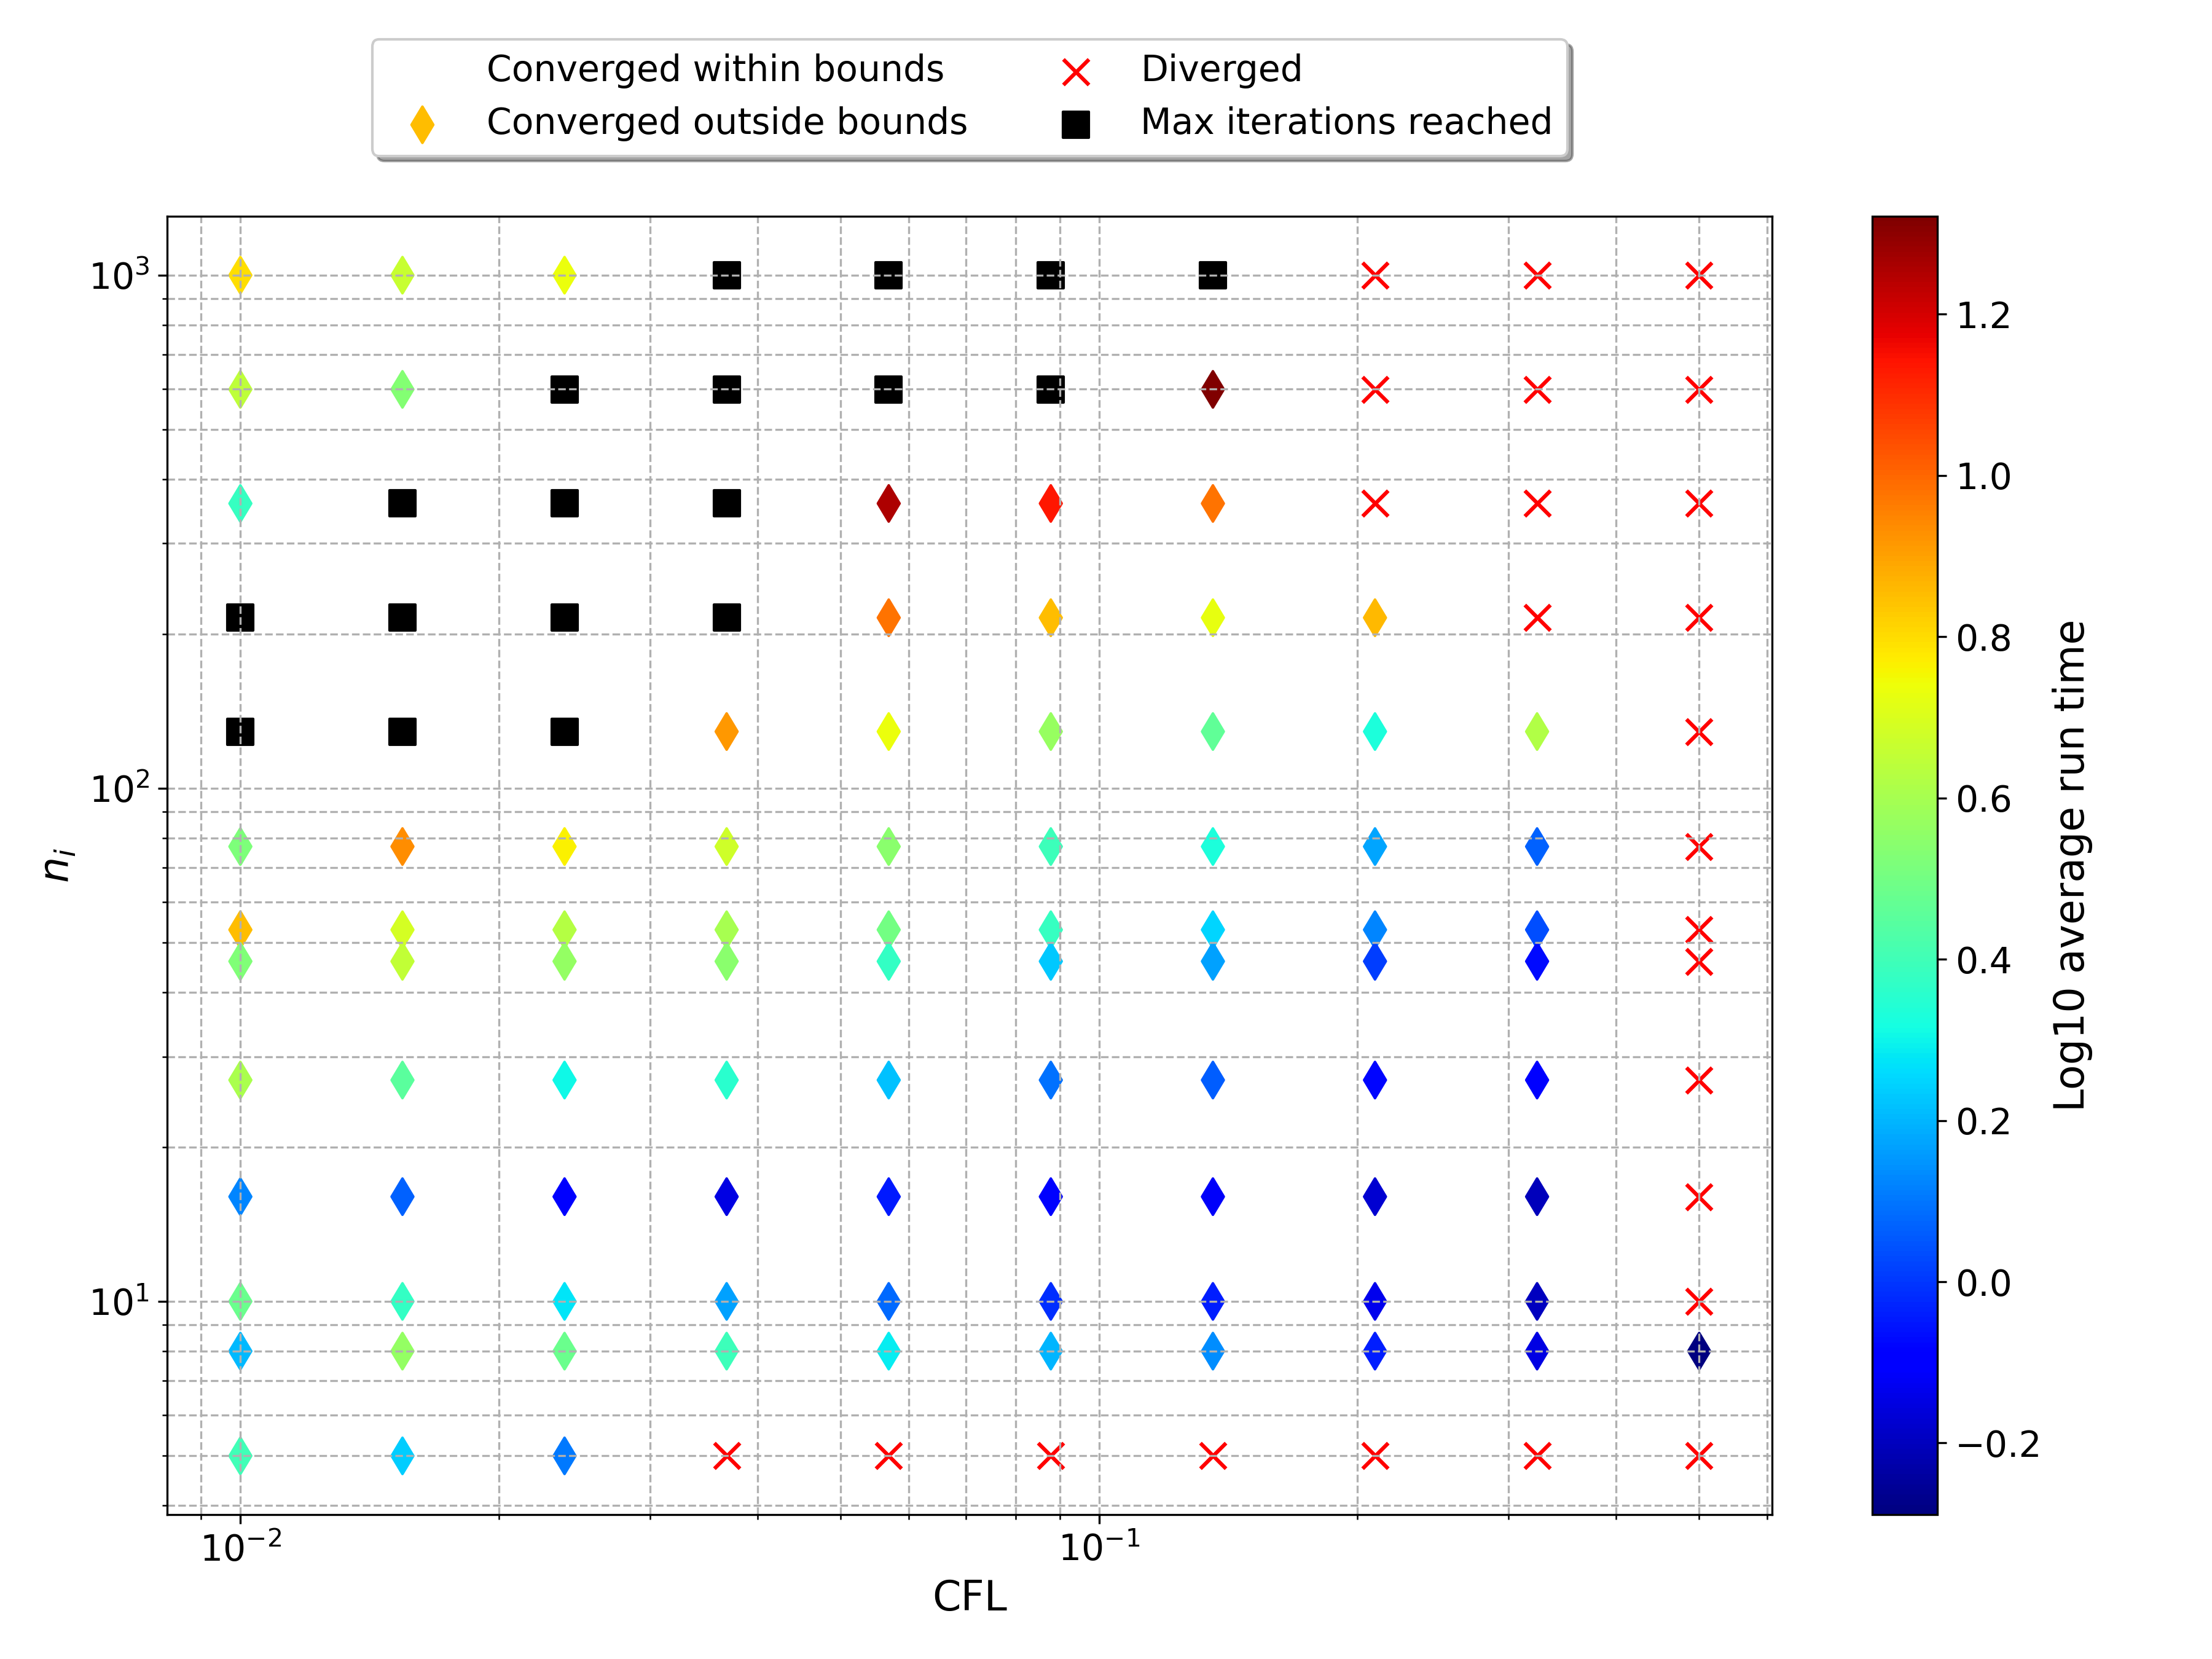
\includegraphics[width=0.8\textwidth]{figures/bump_ni_cfl_time.png}
    \caption{Scatter plot showing variation in runtime for different $CFL$ and $n_i$ values. $sfac = 0.5$. Runs in the top left are incorrectly marked as converged by the solver.}
    \label{fig:bump_ni_cfl_time}
\end{figure}

\subsection{Bend test case}

\begin{figure}[H]
    \centering
    \begin{subfigure}{0.99\textwidth}
        \centering
        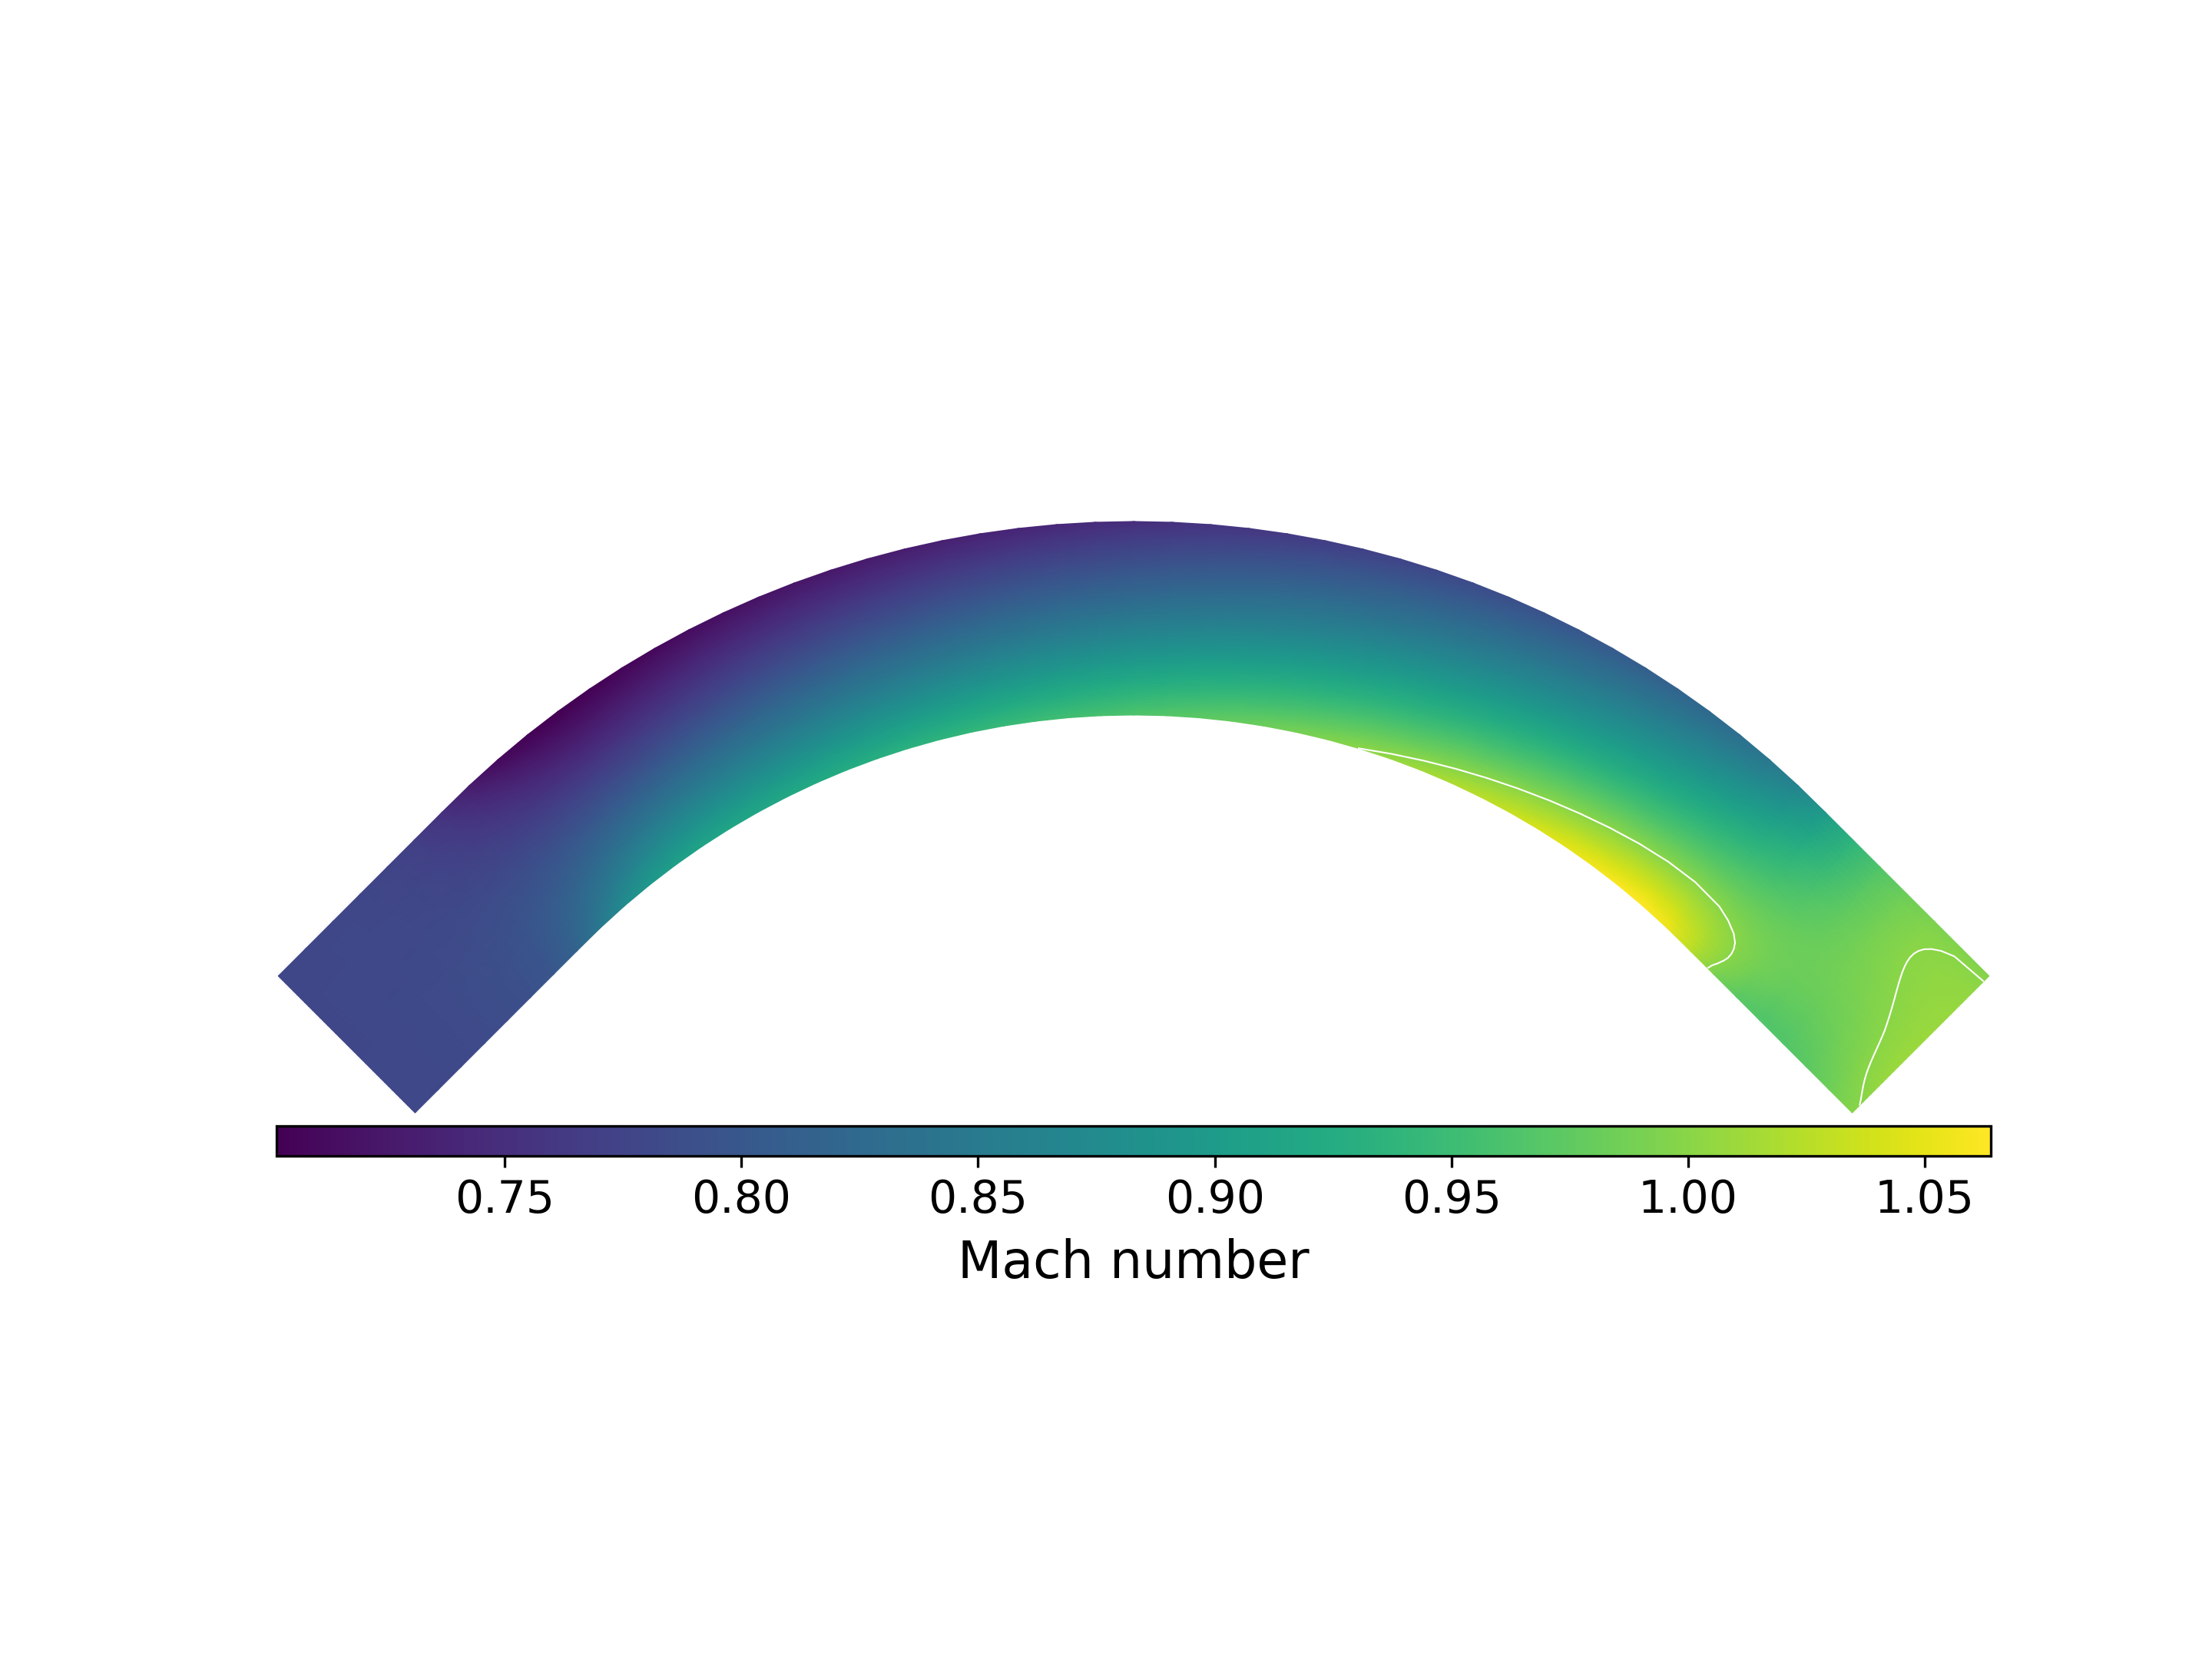
\includegraphics[width=0.7\textwidth]{figures/bend_mach.png}
        \caption{}
        \label{fig:bend_mach}
    \end{subfigure}
    \begin{subfigure}{0.99\textwidth}
        \centering
        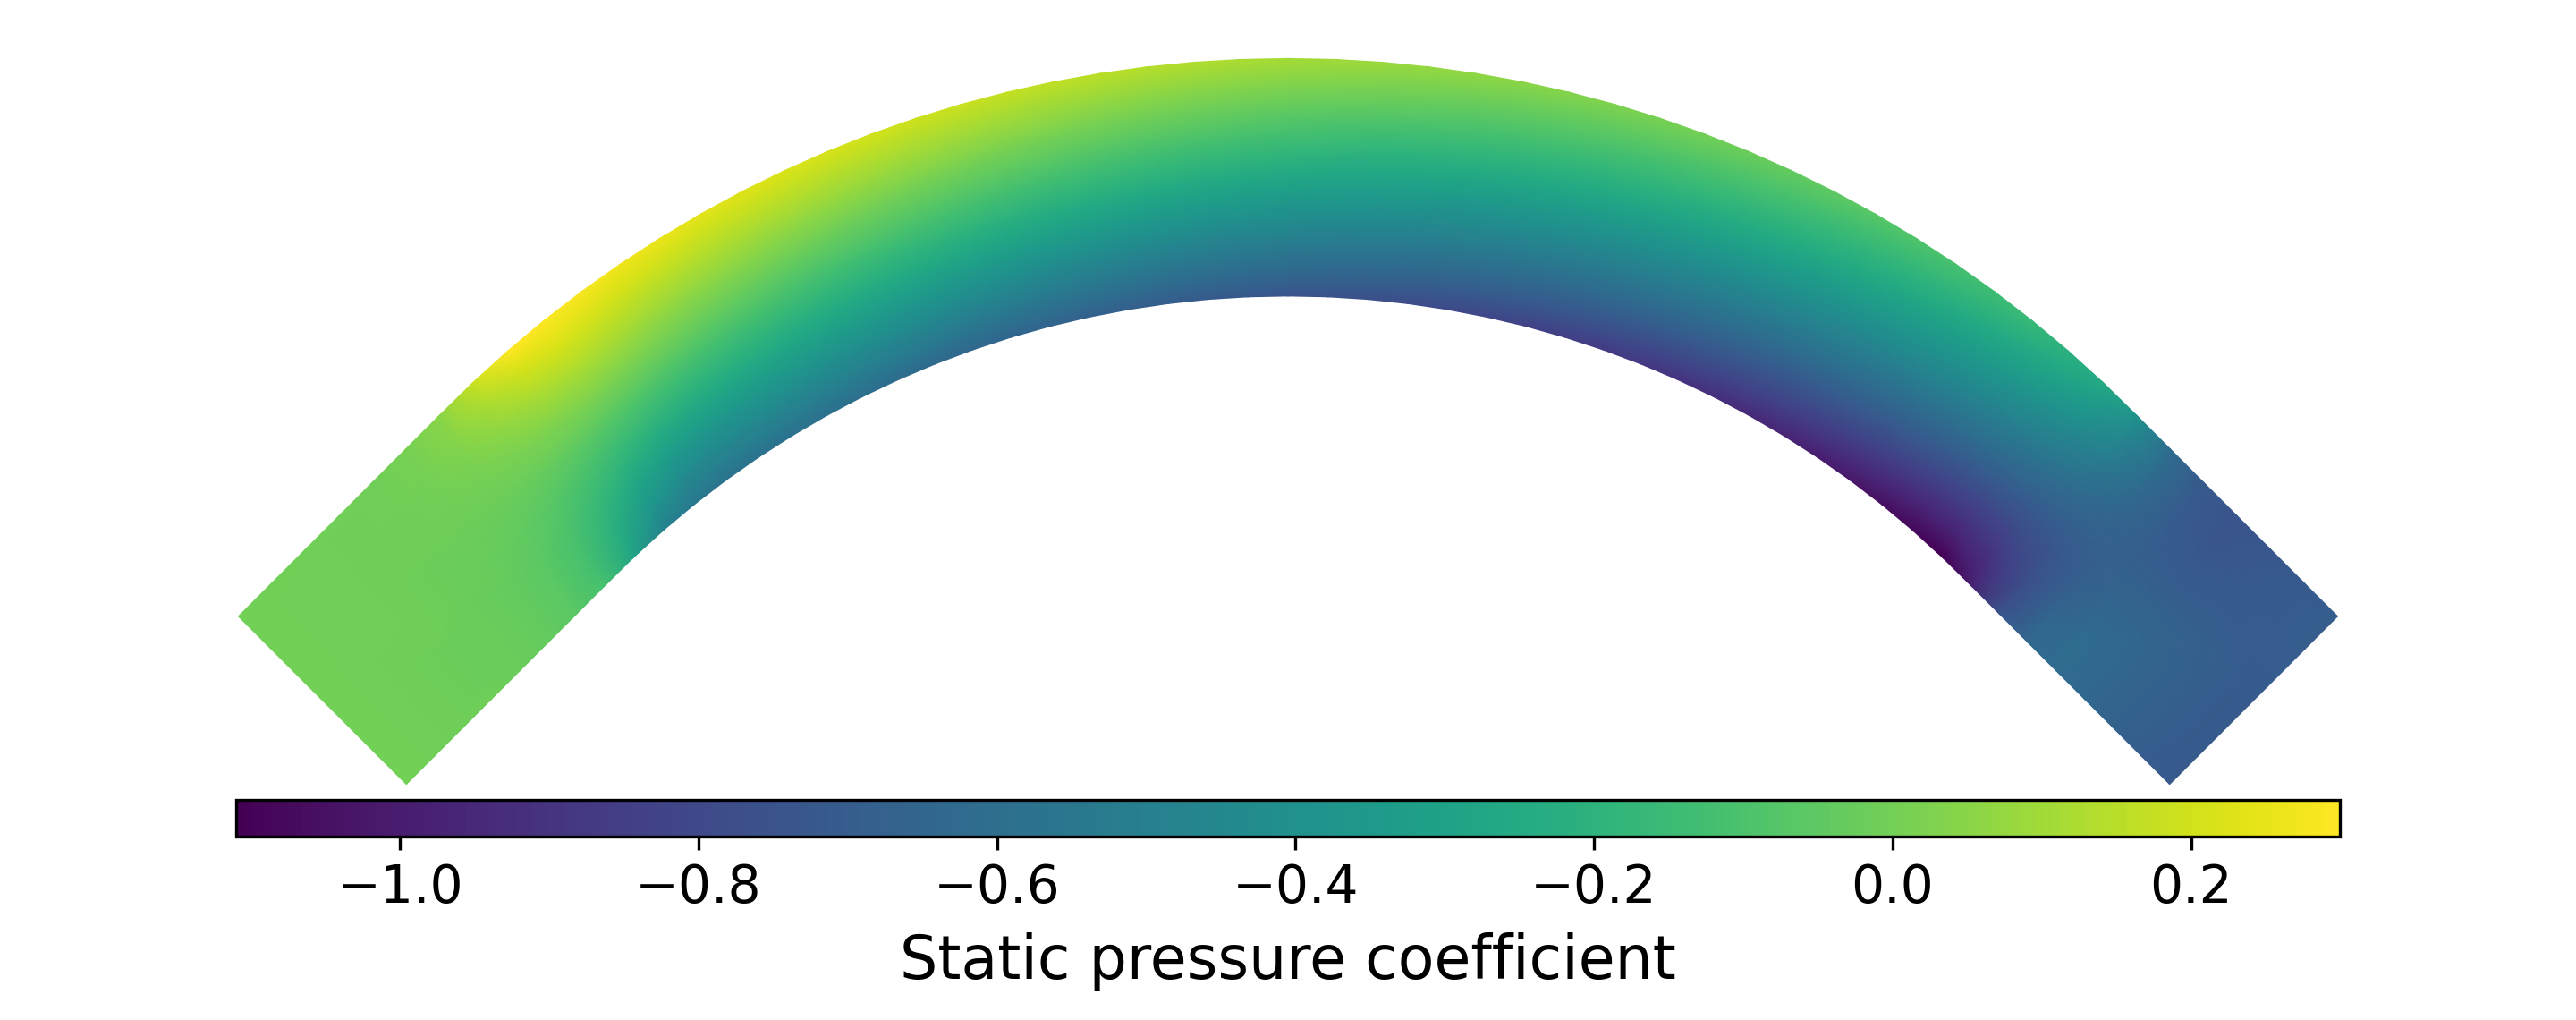
\includegraphics[width=0.7\textwidth]{figures/bend_cp.png}
        \caption{}
        \label{fig:bend_cp}
    \end{subfigure}
    \caption{Bend test case results $CFL = 0.05$, $sfac = 0.1$, $n_i = 53$, $n_j = 37$.}
\end{figure}

\begin{figure}[H]
    \centering
    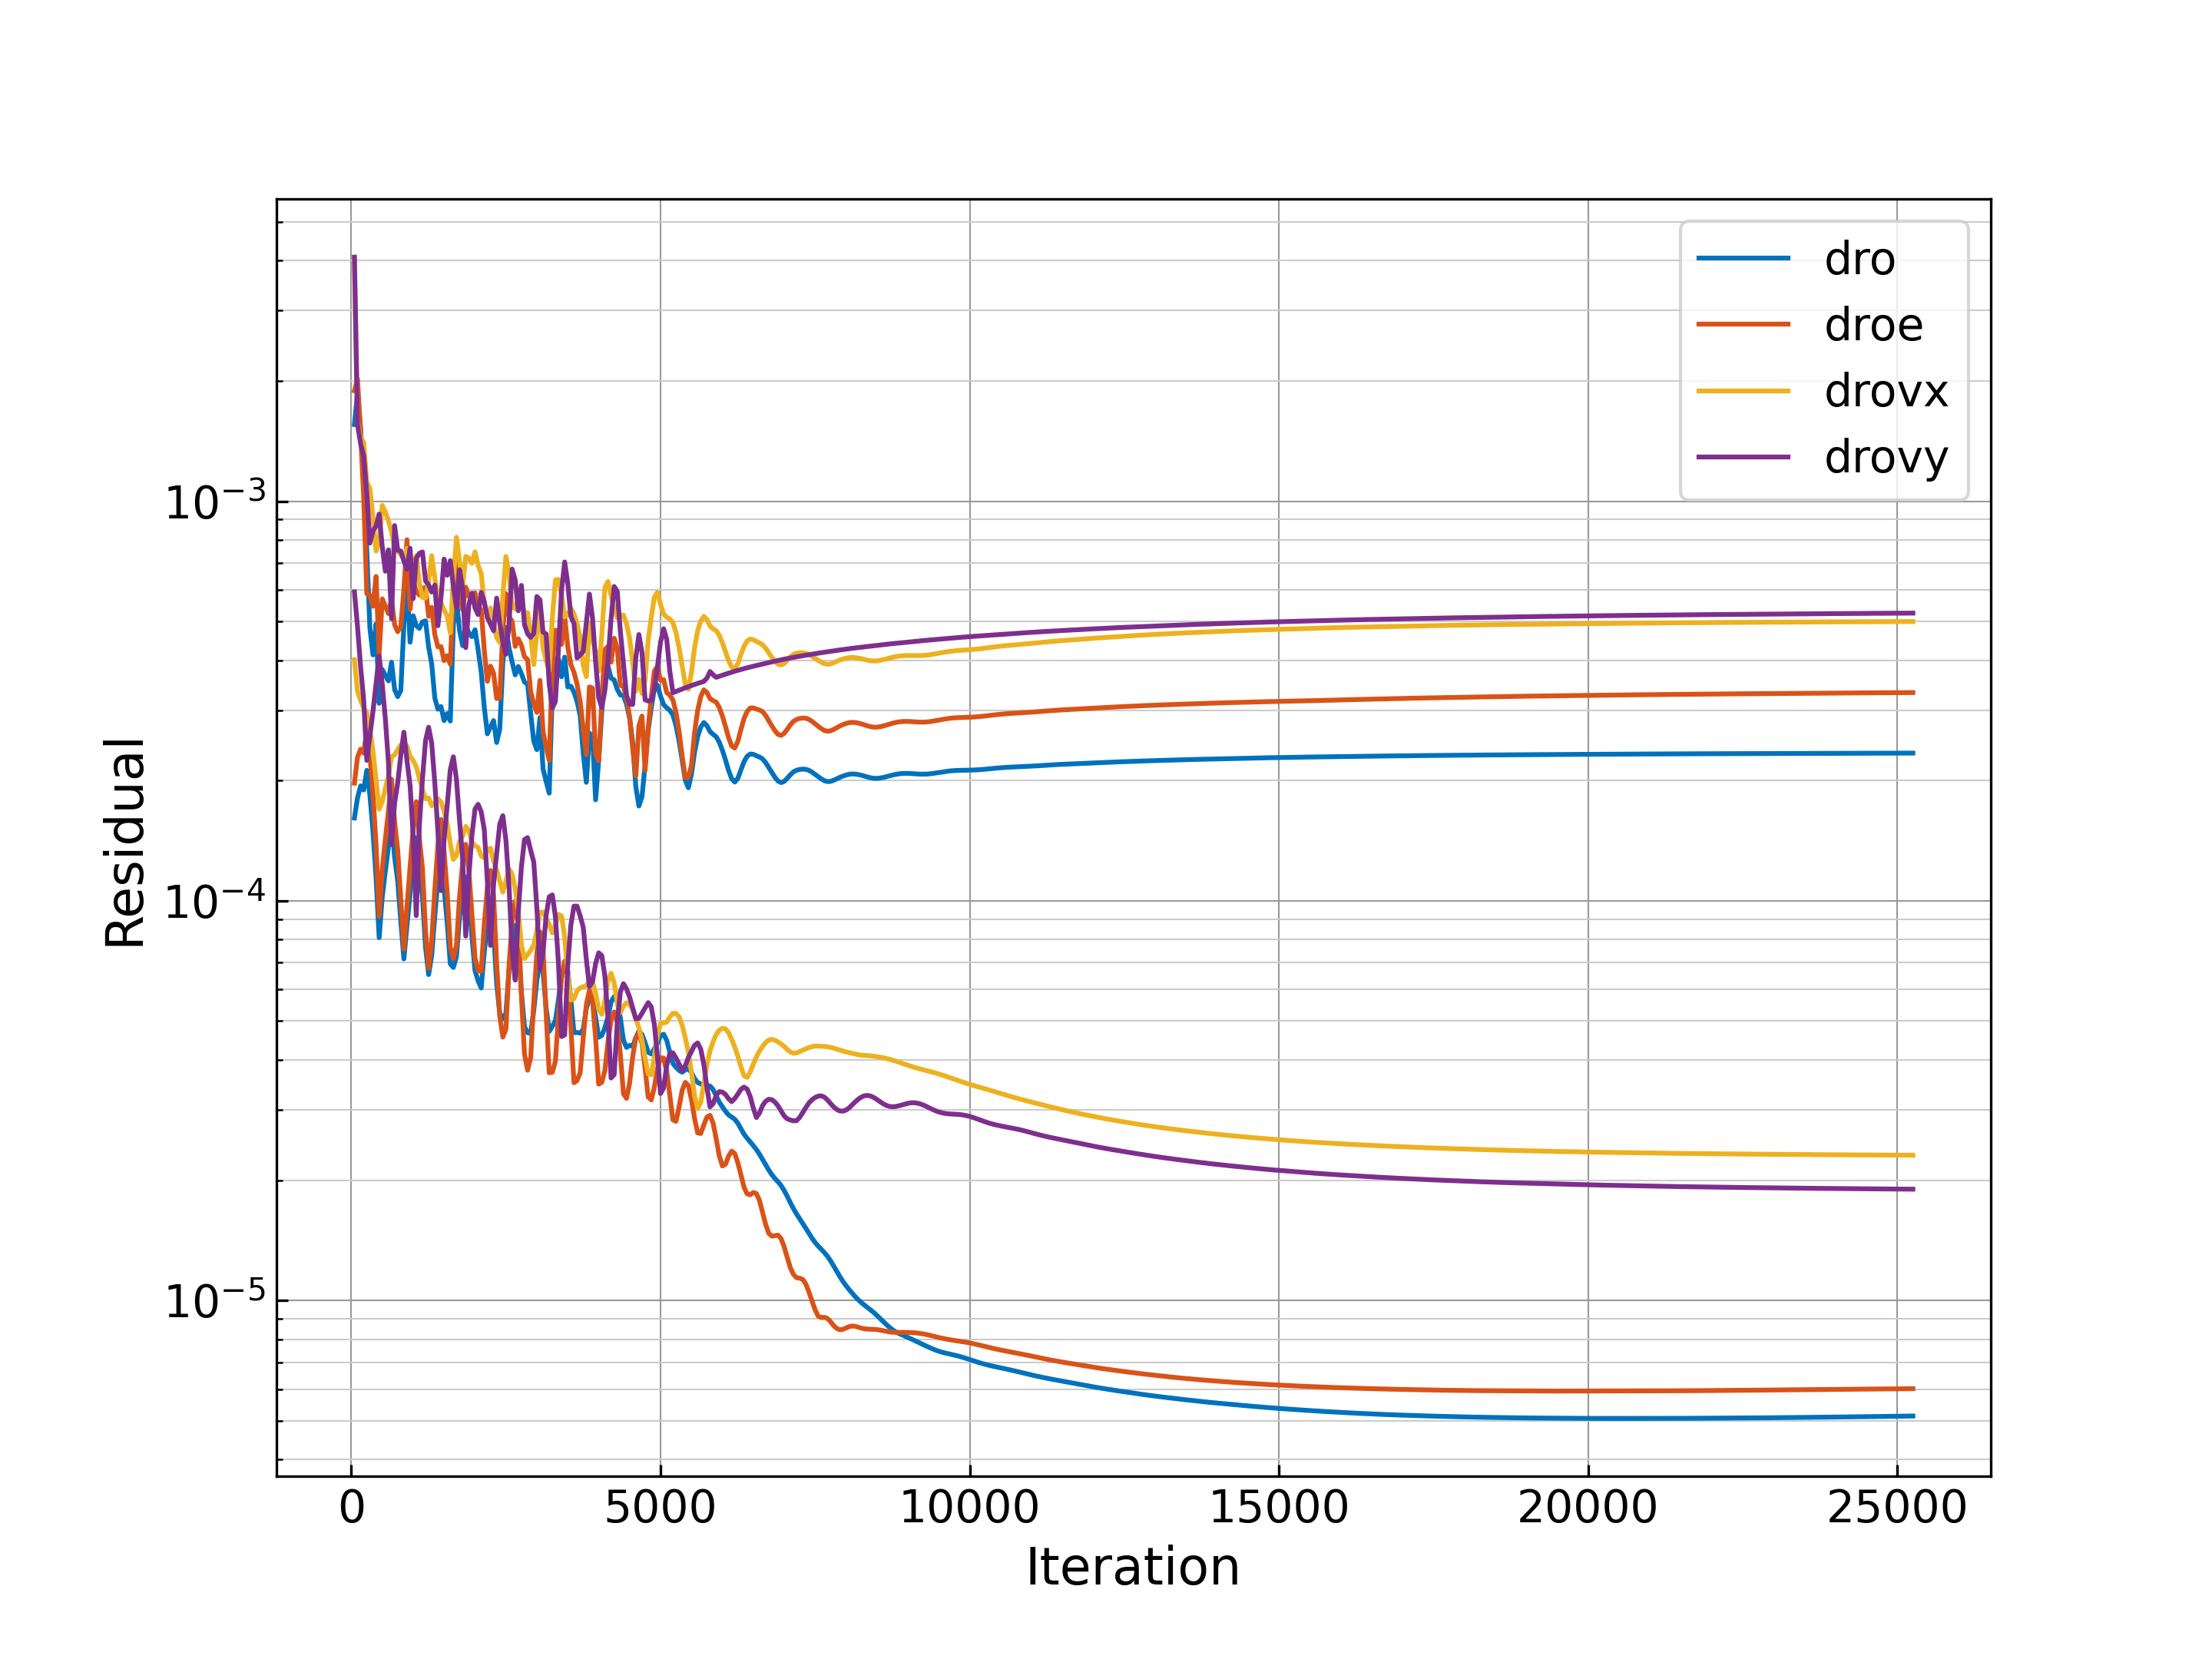
\includegraphics[width=0.7\textwidth]{figures/bend_conv.png}
    \caption{Convergence history of primary flow variables for the bend case}
    \label{fig:bend_conv}
\end{figure}

\begin{figure}[H]
    \centering
    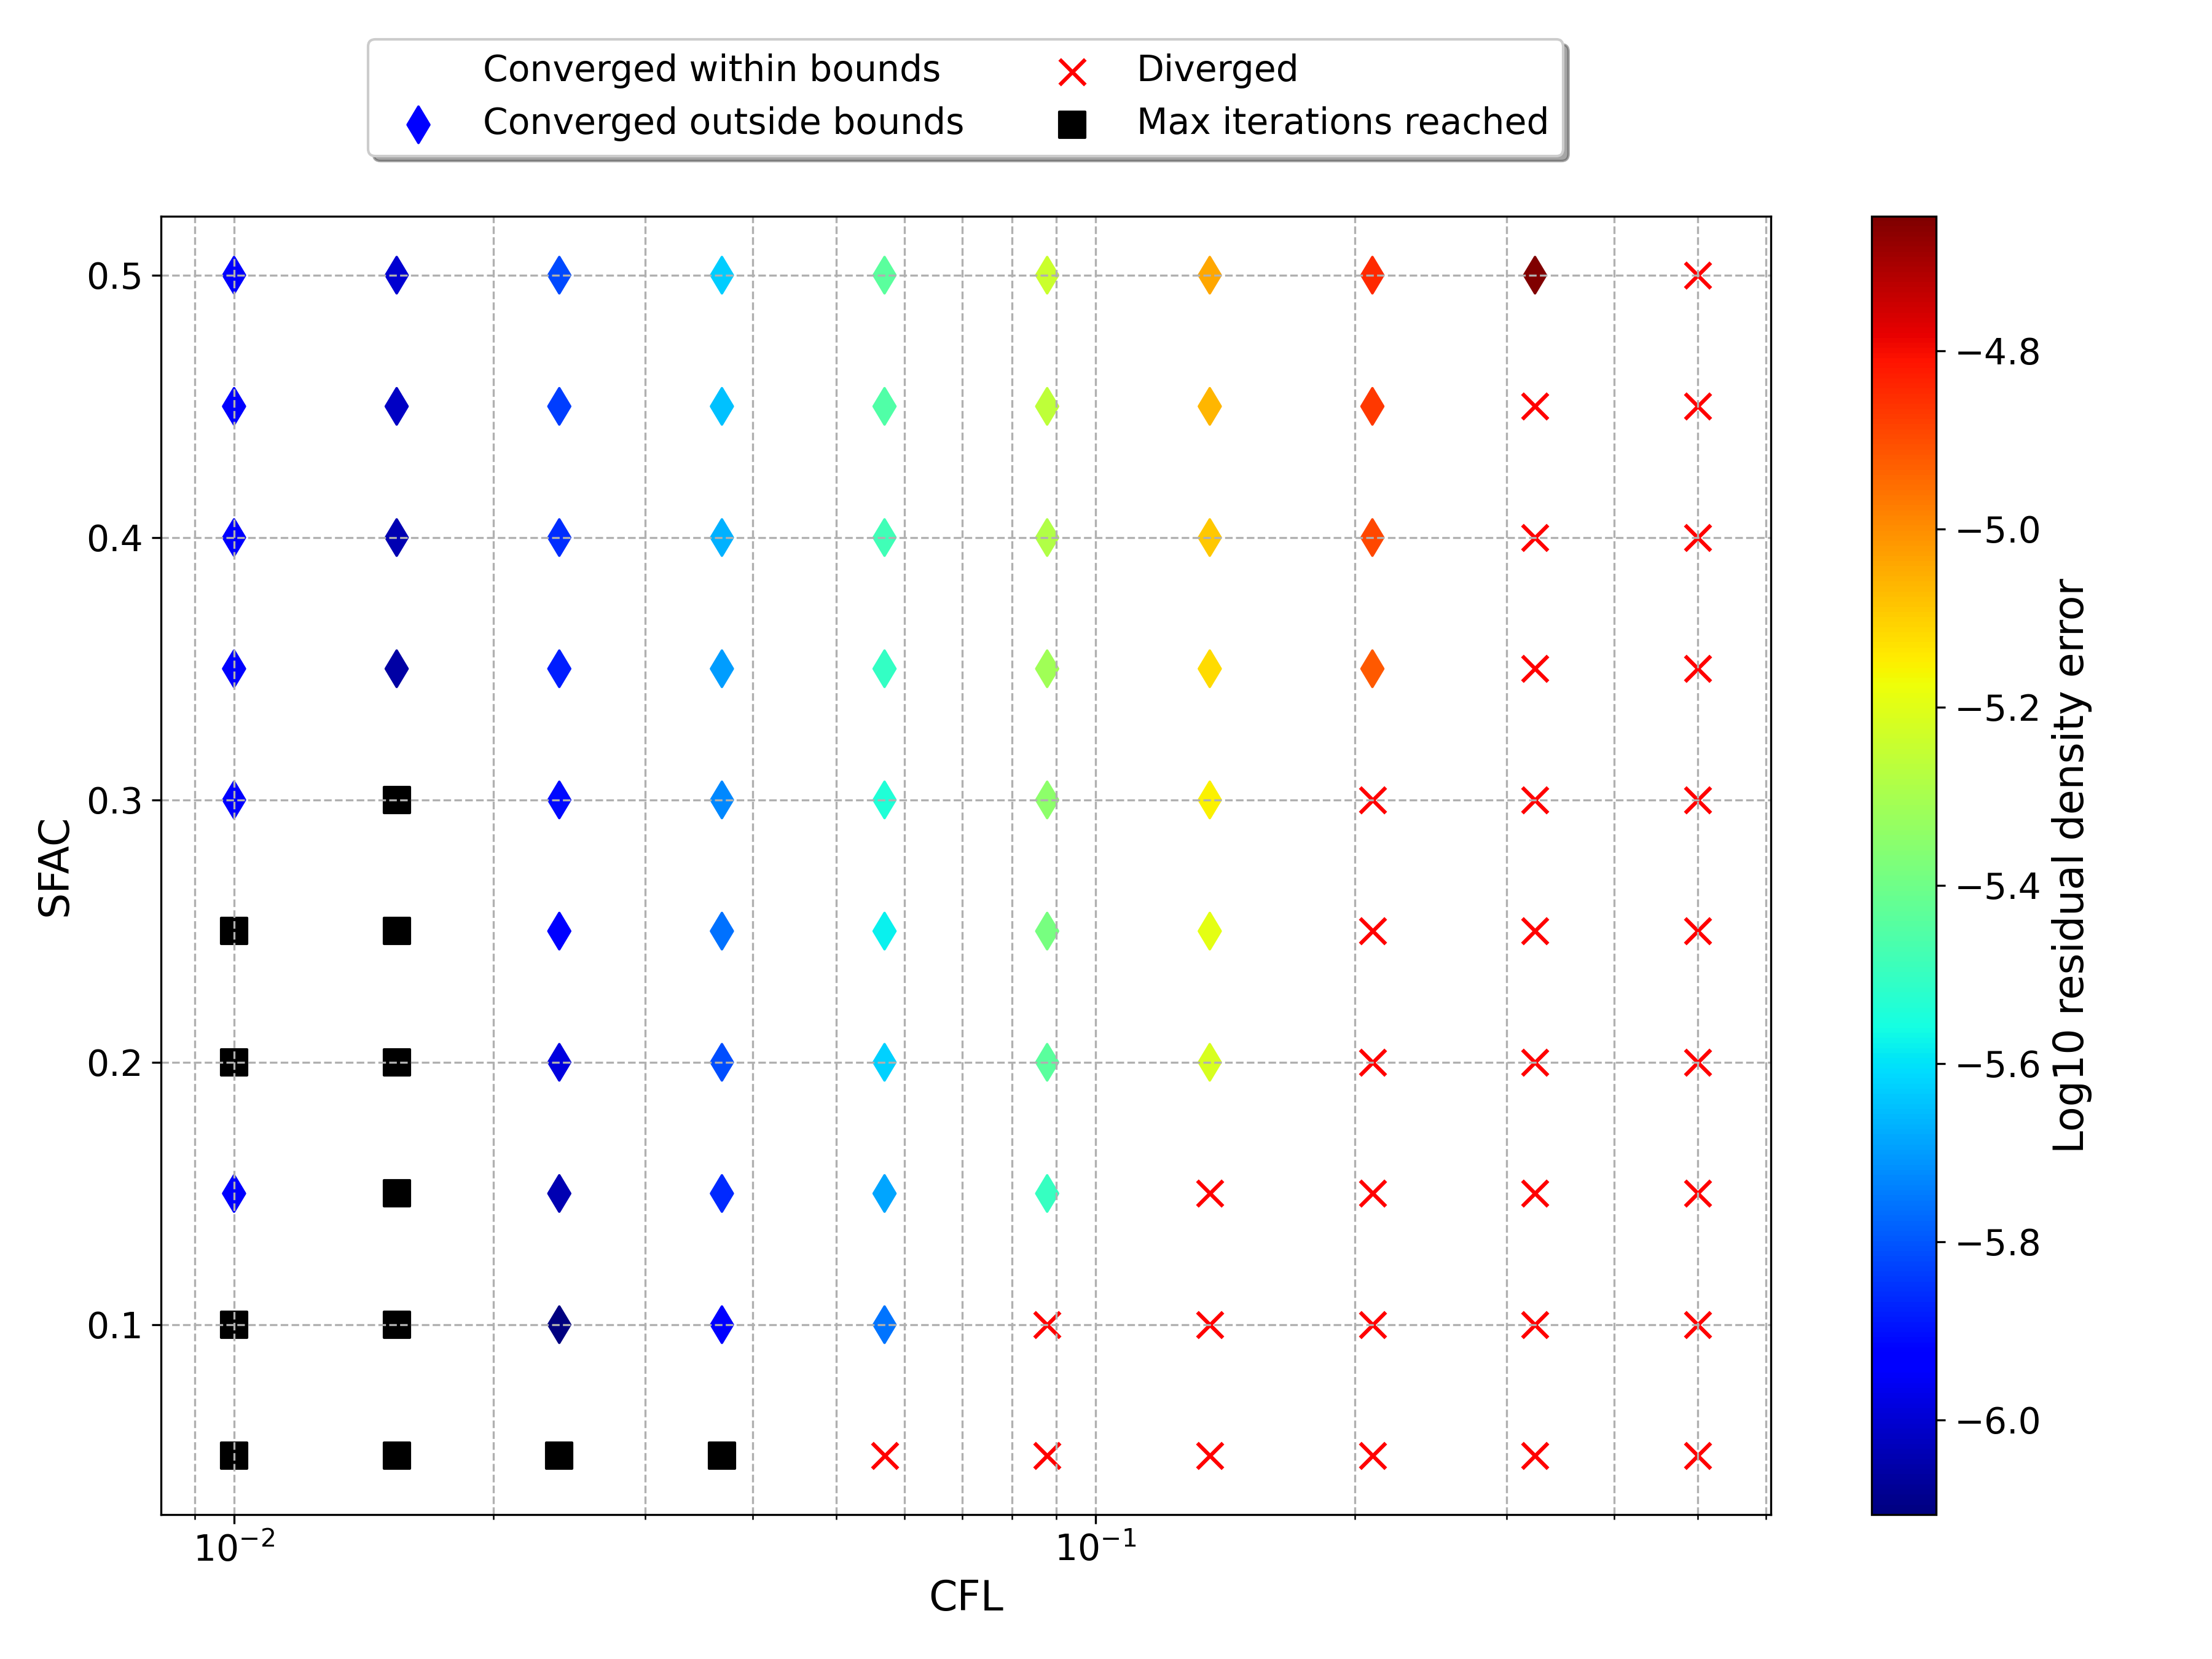
\includegraphics[width=0.8\textwidth]{figures/bend_cfl_sfac_residual.png}
    \caption{Scatter plot showing variation in residual error for different CFL and sfac values.}
    \label{fig:bend_cfl_sfac_residual}
\end{figure}

\begin{figure}[H]
    \centering
    \centering
    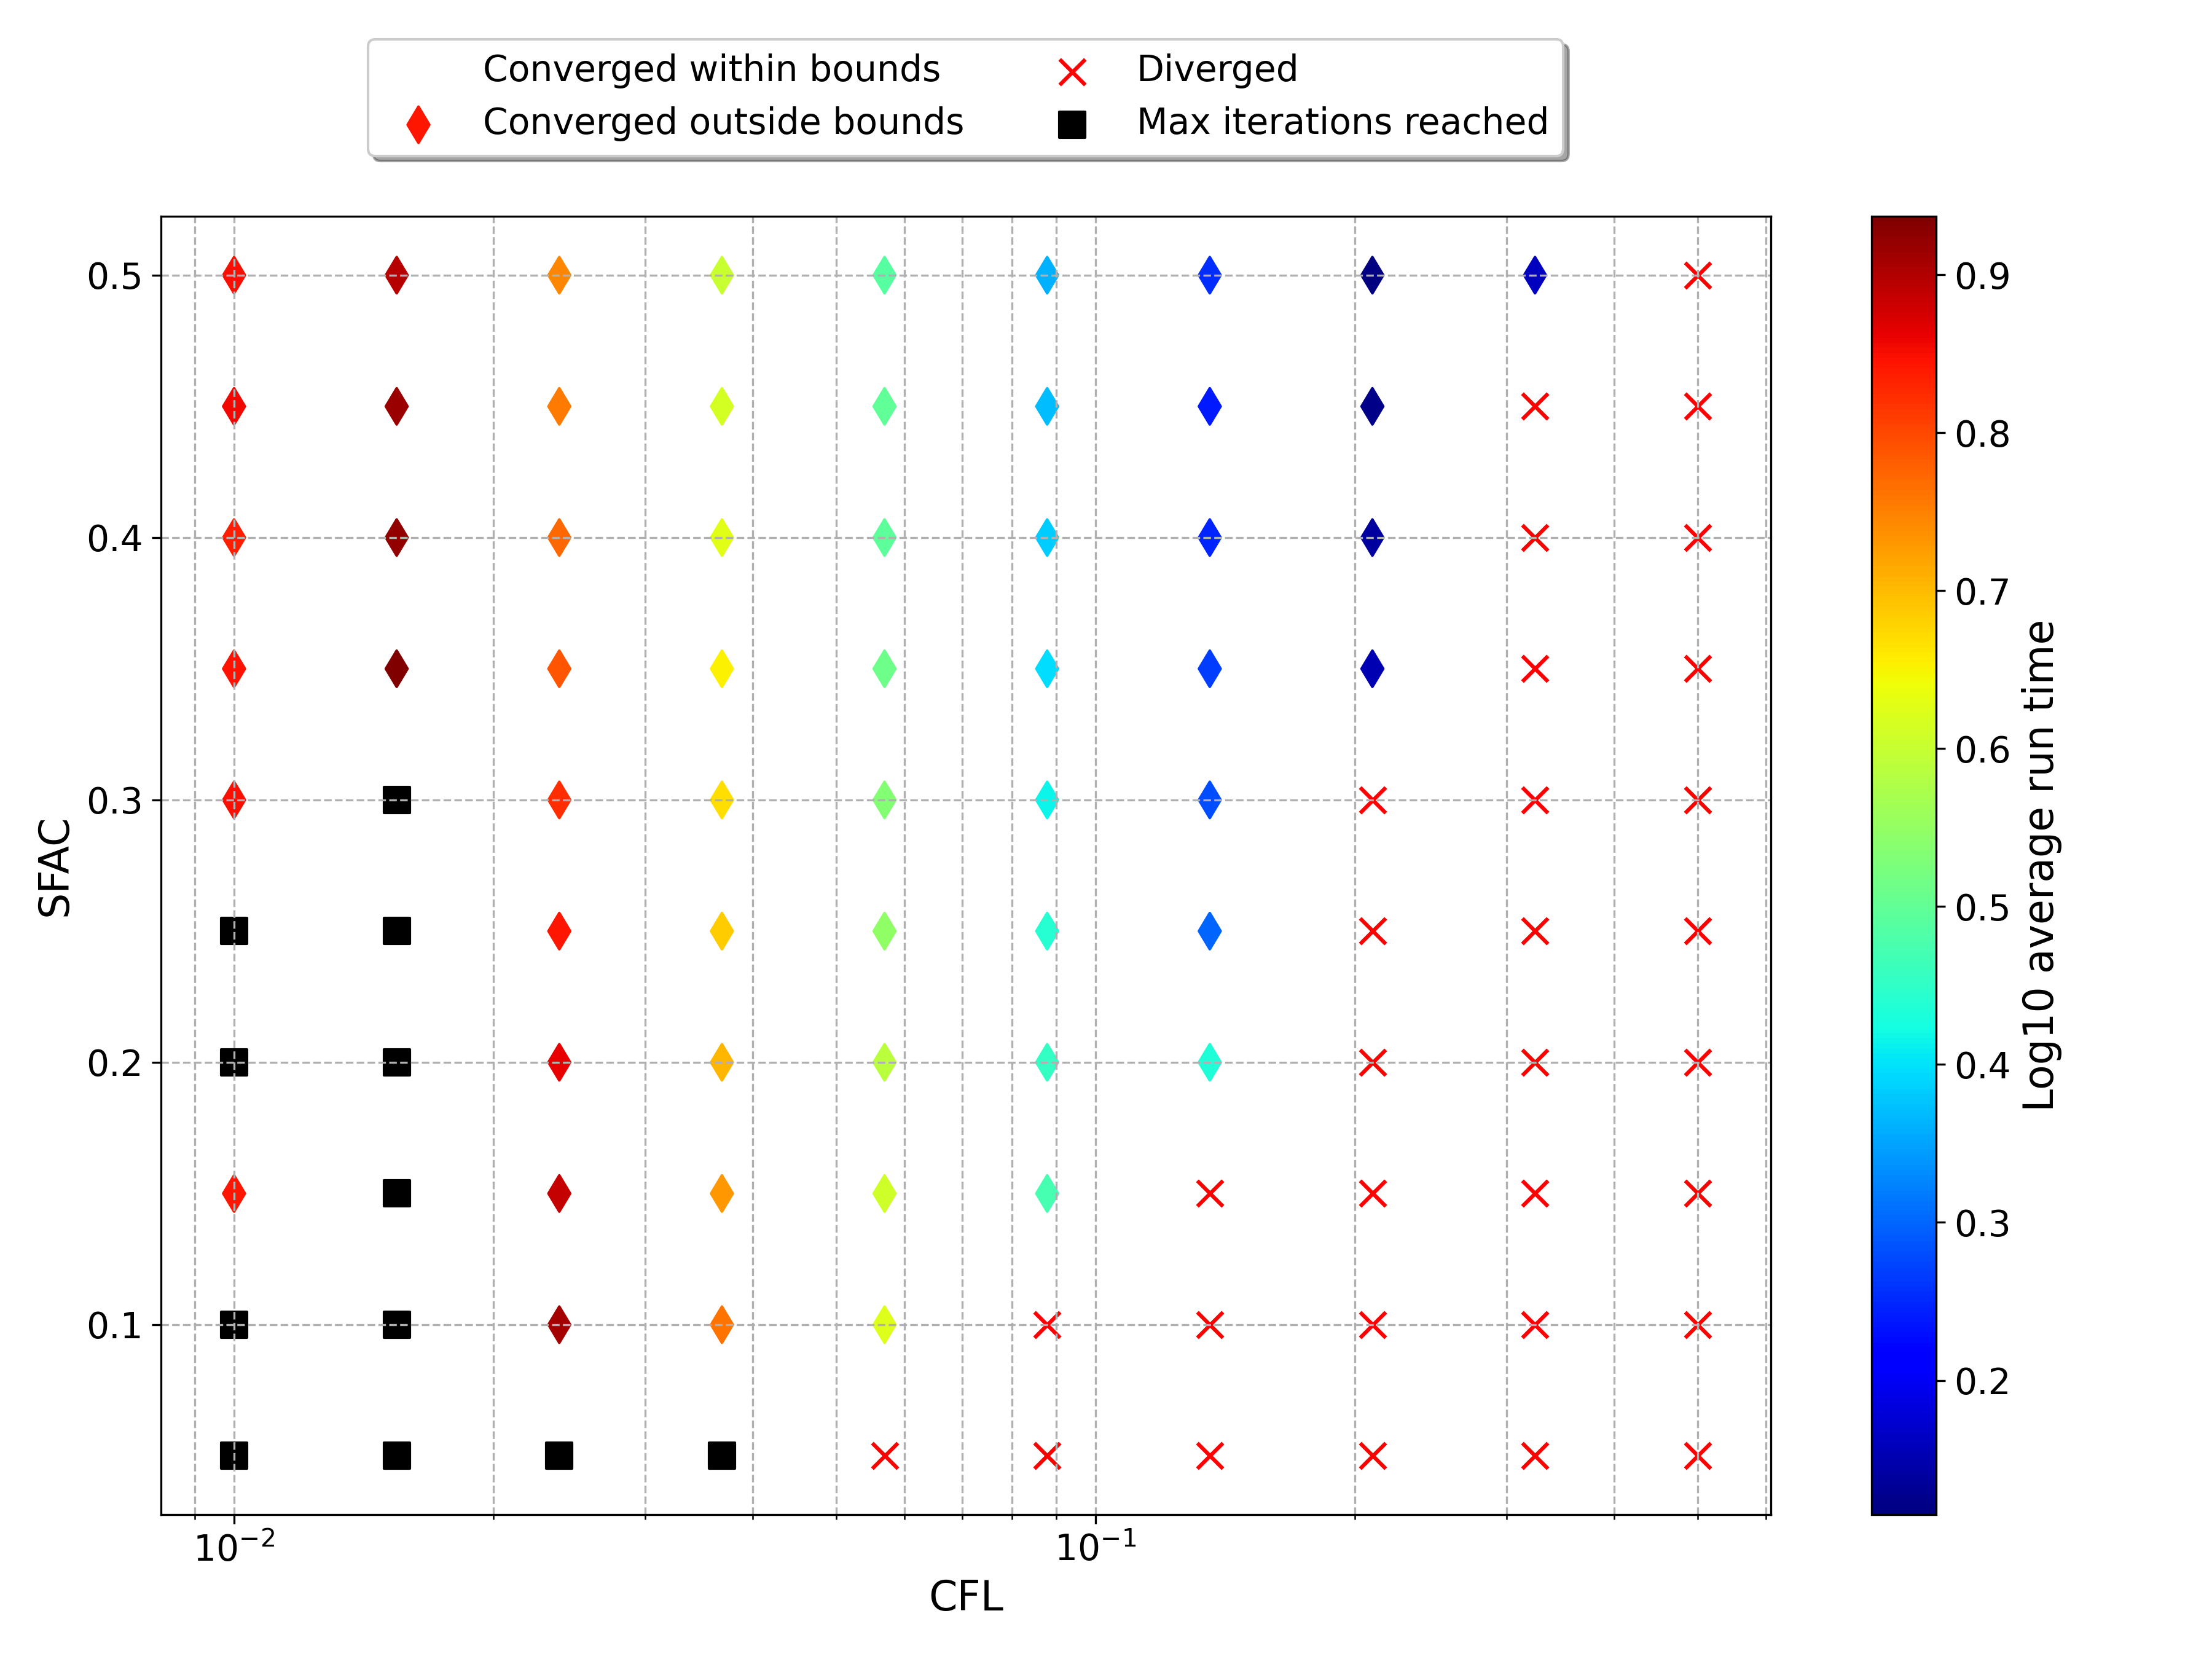
\includegraphics[width=0.8\textwidth]{figures/bend_cfl_sfac_time.png}
    \caption{Scatter plot showing variation in run time for different CFL and sfac values.}
    \label{fig:bend_cfl_sfac_time}
\end{figure}

\subsection{Comparison of compiler options }

\begin{table}[H]
    \centering
    \begin{tabular}{lcc}
        \toprule
        \textbf{Configuration} & \textbf{Normalised Time}  & \textbf{Variation Coefficient} \\
        \midrule
        Debug & 6.83 & 0.021 \\
        Release O2 & 1.05 & 0.018 \\
        Release O2, QxHost & 1.69 & 0.049 \\
        Release O2, Qparallel & 2.66 & 0.087 \\
        Release O2, fp:fast & 1.01 & 0.036 \\
        Release O3 & 1.09 & 0.016 \\
        Release O3, fp:fast & 1.00 & 0.010 \\
        Release O2 & 1.03 & 0.019 \\
        \bottomrule
    \end{tabular}
    \caption{Standard bump case run times for various compiler flags, normalised by the minimum averaged time. The average and deviation were found over three runs at a low $CFL$ such that 20,000 iterations were performed.}
    \label{tab:performance}
\end{table}

\subsection{Device Specifications}

\begin{table}[H]
    \centering
    \begin{tabular}{ll}
        \toprule
        \textbf{Component} & \textbf{Specification} \\
        \midrule
        CPU & AMD Ryzen 9 3900x \\
        GPU & NVIDIA GeForce GTX 1070 \\
        RAM & 32GB DDR4 3200MHz \\
        OS & Windows 10 \\
        \bottomrule
    \end{tabular}
    \caption{Device specifications used for testing.}
    \label{tab:device}
\end{table}

\begin{thebibliography}{9}

  \bibitem{handout}
  J. V. Taylor
  \emph{4A2 COMPUTATIONAL FLUID DYNAMICS: WRITING AN EULER SOLVER}
  University of Cambridge,
  2024.

\end{thebibliography}

\end{document}